
%% bare_conf.tex
%% V1.3
%% 2007/01/11
%% by Michael Shell
%% See:
%% http://www.michaelshell.org/
%% for current contact information.
%%
%% This is a skeleton file demonstrating the use of IEEEtran.cls
%% (requires IEEEtran.cls version 1.7 or later) with an IEEE conference paper.
%%
%% Support sites:
%% http://www.michaelshell.org/tex/ieeetran/
%% http://www.ctan.org/tex-archive/macros/latex/contrib/IEEEtran/
%% and
%% http://www.ieee.org/

%%*************************************************************************
%% Legal Notice:
%% This code is offered as-is without any warranty either expressed or
%% implied; without even the implied warranty of MERCHANTABILITY or
%% FITNESS FOR A PARTICULAR PURPOSE!
%% User assumes all risk.
%% In no event shall IEEE or any contributor to this code be liable for
%% any damages or losses, including, but not limited to, incidental,
%% consequential, or any other damages, resulting from the use or misuse
%% of any information contained here.
%%
%% All comments are the opinions of their respective authors and are not
%% necessarily endorsed by the IEEE.
%%
%% This work is distributed under the LaTeX Project Public License (LPPL)
%% ( http://www.latex-project.org/ ) version 1.3, and may be freely used,
%% distributed and modified. A copy of the LPPL, version 1.3, is included
%% in the base LaTeX documentation of all distributions of LaTeX released
%% 2003/12/01 or later.
%% Retain all contribution notices and credits.
%% ** Modified files should be clearly indicated as such, including  **
%% ** renaming them and changing author support contact information. **
%%
%% File list of work: IEEEtran.cls, IEEEtran_HOWTO.pdf, bare_adv.tex,
%%                    bare_conf.tex, bare_jrnl.tex, bare_jrnl_compsoc.tex
%%*************************************************************************

% *** Authors should verify (and, if needed, correct) their LaTeX system  ***
% *** with the testflow diagnostic prior to trusting their LaTeX platform ***
% *** with production work. IEEE's font choices can trigger bugs that do  ***
% *** not appear when using other class files.                            ***
% The testflow support page is at:
% http://www.michaelshell.org/tex/testflow/



% Note that the a4paper option is mainly intended so that authors in
% countries using A4 can easily print to A4 and see how their papers will
% look in print - the typesetting of the document will not typically be
% affected with changes in paper size (but the bottom and side margins will).
% Use the testflow package mentioned above to verify correct handling of
% both paper sizes by the user's LaTeX system.
%
% Also note that the "draftcls" or "draftclsnofoot", not "draft", option
% should be used if it is desired that the figures are to be displayed in
% draft mode.
%
\documentclass[10pt, conference]{IEEEtran}
% Add the compsocconf option for Computer Society conferences.
%
% If IEEEtran.cls has not been installed into the LaTeX system files,
% manually specify the path to it like:
% \documentclass[conference]{../sty/IEEEtran}





% Some very useful LaTeX packages include:
% (uncomment the ones you want to load)


% *** MISC UTILITY PACKAGES ***
%
%\usepackage{ifpdf}
% Heiko Oberdiek's ifpdf.sty is very useful if you need conditional
% compilation based on whether the output is pdf or dvi.
% usage:
% \ifpdf
%   % pdf code
% \else
%   % dvi code
% \fi
% The latest version of ifpdf.sty can be obtained from:
% http://www.ctan.org/tex-archive/macros/latex/contrib/oberdiek/
% Also, note that IEEEtran.cls V1.7 and later provides a builtin
% \ifCLASSINFOpdf conditional that works the same way.
% When switching from latex to pdflatex and vice-versa, the compiler may
% have to be run twice to clear warning/error messages.






% *** CITATION PACKAGES ***
%
%\usepackage{cite}
% cite.sty was written by Donald Arseneau
% V1.6 and later of IEEEtran pre-defines the format of the cite.sty package
% \cite{} output to follow that of IEEE. Loading the cite package will
% result in citation numbers being automatically sorted and properly
% "compressed/ranged". e.g., [1], [9], [2], [7], [5], [6] without using
% cite.sty will become [1], [2], [5]--[7], [9] using cite.sty. cite.sty's
% \cite will automatically add leading space, if needed. Use cite.sty's
% noadjust option (cite.sty V3.8 and later) if you want to turn this off.
% cite.sty is already installed on most LaTeX systems. Be sure and use
% version 4.0 (2003-05-27) and later if using hyperref.sty. cite.sty does
% not currently provide for hyperlinked citations.
% The latest version can be obtained at:
% http://www.ctan.org/tex-archive/macros/latex/contrib/cite/
% The documentation is contained in the cite.sty file itself.






% *** GRAPHICS RELATED PACKAGES ***
%
\ifCLASSINFOpdf
  % \usepackage[pdftex]{graphicx}
  % declare the path(s) where your graphic files are
  % \graphicspath{{../pdf/}{../jpeg/}}
  % and their extensions so you won't have to specify these with
  % every instance of \includegraphics
  % \DeclareGraphicsExtensions{.pdf,.jpeg,.png}
\else
  % or other class option (dvipsone, dvipdf, if not using dvips). graphicx
  % will default to the driver specified in the system graphics.cfg if no
  % driver is specified.
  % \usepackage[dvips]{graphicx}
  % declare the path(s) where your graphic files are
  % \graphicspath{{../eps/}}
  % and their extensions so you won't have to specify these with
  % every instance of \includegraphics
  % \DeclareGraphicsExtensions{.eps}
\fi
% graphicx was written by David Carlisle and Sebastian Rahtz. It is
% required if you want graphics, photos, etc. graphicx.sty is already
% installed on most LaTeX systems. The latest version and documentation can
% be obtained at:
% http://www.ctan.org/tex-archive/macros/latex/required/graphics/
% Another good source of documentation is "Using Imported Graphics in
% LaTeX2e" by Keith Reckdahl which can be found as epslatex.ps or
% epslatex.pdf at: http://www.ctan.org/tex-archive/info/
%
% latex, and pdflatex in dvi mode, support graphics in encapsulated
% postscript (.eps) format. pdflatex in pdf mode supports graphics
% in .pdf, .jpeg, .png and .mps (metapost) formats. Users should ensure
% that all non-photo figures use a vector format (.eps, .pdf, .mps) and
% not a bitmapped formats (.jpeg, .png). IEEE frowns on bitmapped formats
% which can result in "jaggedy"/blurry rendering of lines and letters as
% well as large increases in file sizes.
%
% You can find documentation about the pdfTeX application at:
% http://www.tug.org/applications/pdftex





% *** MATH PACKAGES ***
%
%\usepackage[cmex10]{amsmath}
% A popular package from the American Mathematical Society that provides
% many useful and powerful commands for dealing with mathematics. If using
% it, be sure to load this package with the cmex10 option to ensure that
% only type 1 fonts will utilized at all point sizes. Without this option,
% it is possible that some math symbols, particularly those within
% footnotes, will be rendered in bitmap form which will result in a
% document that can not be IEEE Xplore compliant!
%
% Also, note that the amsmath package sets \interdisplaylinepenalty to 10000
% thus preventing page breaks from occurring within multiline equations. Use:
%\interdisplaylinepenalty=2500
% after loading amsmath to restore such page breaks as IEEEtran.cls normally
% does. amsmath.sty is already installed on most LaTeX systems. The latest
% version and documentation can be obtained at:
% http://www.ctan.org/tex-archive/macros/latex/required/amslatex/math/





% *** SPECIALIZED LIST PACKAGES ***
%
%\usepackage{algorithmic}
% algorithmic.sty was written by Peter Williams and Rogerio Brito.
% This package provides an algorithmic environment fo describing algorithms.
% You can use the algorithmic environment in-text or within a figure
% environment to provide for a floating algorithm. Do NOT use the algorithm
% floating environment provided by algorithm.sty (by the same authors) or
% algorithm2e.sty (by Christophe Fiorio) as IEEE does not use dedicated
% algorithm float types and packages that provide these will not provide
% correct IEEE style captions. The latest version and documentation of
% algorithmic.sty can be obtained at:
% http://www.ctan.org/tex-archive/macros/latex/contrib/algorithms/
% There is also a support site at:
% http://algorithms.berlios.de/index.html
% Also of interest may be the (relatively newer and more customizable)
% algorithmicx.sty package by Szasz Janos:
% http://www.ctan.org/tex-archive/macros/latex/contrib/algorithmicx/




% *** ALIGNMENT PACKAGES ***
%
%\usepackage{array}
% Frank Mittelbach's and David Carlisle's array.sty patches and improves
% the standard LaTeX2e array and tabular environments to provide better
% appearance and additional user controls. As the default LaTeX2e table
% generation code is lacking to the point of almost being broken with
% respect to the quality of the end results, all users are strongly
% advised to use an enhanced (at the very least that provided by array.sty)
% set of table tools. array.sty is already installed on most systems. The
% latest version and documentation can be obtained at:
% http://www.ctan.org/tex-archive/macros/latex/required/tools/


%\usepackage{mdwmath}
%\usepackage{mdwtab}
% Also highly recommended is Mark Wooding's extremely powerful MDW tools,
% especially mdwmath.sty and mdwtab.sty which are used to format equations
% and tables, respectively. The MDWtools set is already installed on most
% LaTeX systems. The lastest version and documentation is available at:
% http://www.ctan.org/tex-archive/macros/latex/contrib/mdwtools/


% IEEEtran contains the IEEEeqnarray family of commands that can be used to
% generate multiline equations as well as matrices, tables, etc., of high
% quality.


%\usepackage{eqparbox}
% Also of notable interest is Scott Pakin's eqparbox package for creating
% (automatically sized) equal width boxes - aka "natural width parboxes".
% Available at:
% http://www.ctan.org/tex-archive/macros/latex/contrib/eqparbox/





% *** SUBFIGURE PACKAGES ***
%\usepackage[tight,footnotesize]{subfigure}
% subfigure.sty was written by Steven Douglas Cochran. This package makes it
% easy to put subfigures in your figures. e.g., "Figure 1a and 1b". For IEEE
% work, it is a good idea to load it with the tight package option to reduce
% the amount of white space around the subfigures. subfigure.sty is already
% installed on most LaTeX systems. The latest version and documentation can
% be obtained at:
% http://www.ctan.org/tex-archive/obsolete/macros/latex/contrib/subfigure/
% subfigure.sty has been superceeded by subfig.sty.



%\usepackage[caption=false]{caption}
%\usepackage[font=footnotesize]{subfig}
% subfig.sty, also written by Steven Douglas Cochran, is the modern
% replacement for subfigure.sty. However, subfig.sty requires and
% automatically loads Axel Sommerfeldt's caption.sty which will override
% IEEEtran.cls handling of captions and this will result in nonIEEE style
% figure/table captions. To prevent this problem, be sure and preload
% caption.sty with its "caption=false" package option. This is will preserve
% IEEEtran.cls handing of captions. Version 1.3 (2005/06/28) and later
% (recommended due to many improvements over 1.2) of subfig.sty supports
% the caption=false option directly:
%\usepackage[caption=false,font=footnotesize]{subfig}
%
% The latest version and documentation can be obtained at:
% http://www.ctan.org/tex-archive/macros/latex/contrib/subfig/
% The latest version and documentation of caption.sty can be obtained at:
% http://www.ctan.org/tex-archive/macros/latex/contrib/caption/




% *** FLOAT PACKAGES ***
%
%\usepackage{fixltx2e}
% fixltx2e, the successor to the earlier fix2col.sty, was written by
% Frank Mittelbach and David Carlisle. This package corrects a few problems
% in the LaTeX2e kernel, the most notable of which is that in current
% LaTeX2e releases, the ordering of single and double column floats is not
% guaranteed to be preserved. Thus, an unpatched LaTeX2e can allow a
% single column figure to be placed prior to an earlier double column
% figure. The latest version and documentation can be found at:
% http://www.ctan.org/tex-archive/macros/latex/base/



%\usepackage{stfloats}
% stfloats.sty was written by Sigitas Tolusis. This package gives LaTeX2e
% the ability to do double column floats at the bottom of the page as well
% as the top. (e.g., "\begin{figure*}[!b]" is not normally possible in
% LaTeX2e). It also provides a command:
%\fnbelowfloat
% to enable the placement of footnotes below bottom floats (the standard
% LaTeX2e kernel puts them above bottom floats). This is an invasive package
% which rewrites many portions of the LaTeX2e float routines. It may not work
% with other packages that modify the LaTeX2e float routines. The latest
% version and documentation can be obtained at:
% http://www.ctan.org/tex-archive/macros/latex/contrib/sttools/
% Documentation is contained in the stfloats.sty comments as well as in the
% presfull.pdf file. Do not use the stfloats baselinefloat ability as IEEE
% does not allow \baselineskip to stretch. Authors submitting work to the
% IEEE should note that IEEE rarely uses double column equations and
% that authors should try to avoid such use. Do not be tempted to use the
% cuted.sty or midfloat.sty packages (also by Sigitas Tolusis) as IEEE does
% not format its papers in such ways.





% *** PDF, URL AND HYPERLINK PACKAGES ***
%
%\usepackage{url}
% url.sty was written by Donald Arseneau. It provides better support for
% handling and breaking URLs. url.sty is already installed on most LaTeX
% systems. The latest version can be obtained at:
% http://www.ctan.org/tex-archive/macros/latex/contrib/misc/
% Read the url.sty source comments for usage information. Basically,
% \url{my_url_here}.





% *** Do not adjust lengths that control margins, column widths, etc. ***
% *** Do not use packages that alter fonts (such as pslatex).         ***
% There should be no need to do such things with IEEEtran.cls V1.6 and later.
% (Unless specifically asked to do so by the journal or conference you plan
% to submit to, of course. )


% correct bad hyphenation here
\hyphenation{op-tical net-works semi-conduc-tor}

%\usepackage{ulem}
%\usepackage{latex8}
%\usepackage{times}
\usepackage{epsf}
%\usepackage[utf8]{vietnam}
%\usepackage{latexsym}
%\usepackage{tweaklist}
\usepackage{graphicx}
\usepackage{rotating}
\usepackage{booktabs}
\usepackage{ctable}
\usepackage{listings}
\usepackage{alltt}
%\usepackage{fvrb-ex}
\lstset{basicstyle=\scriptsize\sffamily,language=Pascal,tabsize=2,frame=single,breaklines=true,columns=flexible,mathescape=true,showspaces=false,showstringspaces=false,showtabs=false}

\begin{document}

\newtheorem{Definition}{Definition}
\newtheorem{Claim}{Claim}
\newtheorem{Lemma}{Lemma}
\newtheorem{Theorem}{Theorem}
\newtheorem{Property}{Property}
\newcommand{\code}[1]{{\footnotesize\textsf{#1}}}

\newcommand{\tool} {iTrack}
\newcommand{\concept} {feature}
\newcommand{\users} {users}
\newcommand{\lTypes}{lTypes}

%
% paper title
% can use linebreaks \\ within to get better formatting as desired
\title{Interaction-based Tracking of Program Entities for Repairing
Method Calls in Existing Test Cases}


% author names and affiliations
% use a multiple column layout for up to two different
% affiliations

\author{\IEEEauthorblockN{Hoan Anh Nguyen, Tung Thanh Nguyen, Hung V. Nguyen, and Tien N. Nguyen}
\IEEEauthorblockA{Electrical and Computer Engineering Department\\
Iowa State University \\
\{hoan,tung,hungnv,tien\}@iastate.edu}}

% conference papers do not typically use \thanks and this command
% is locked out in conference mode. If really needed, such as for
% the acknowledgment of grants, issue a \IEEEoverridecommandlockouts
% after \documentclass

% for over three affiliations, or if they all won't fit within the width
% of the page, use this alternative format:
%
%\author{\IEEEauthorblockN{Michael Shell\IEEEauthorrefmark{1},
%Homer Simpson\IEEEauthorrefmark{2},
%James Kirk\IEEEauthorrefmark{3},
%Montgomery Scott\IEEEauthorrefmark{3} and
%Eldon Tyrell\IEEEauthorrefmark{4}}
%\IEEEauthorblockA{\IEEEauthorrefmark{1}School of Electrical and Computer Engineering\\
%Georgia Institute of Technology,
%Atlanta, Georgia 30332--0250\\ Email: see http://www.michaelshell.org/contact.html}
%\IEEEauthorblockA{\IEEEauthorrefmark{2}Twentieth Century Fox, Springfield, USA\\
%Email: homer@thesimpsons.com}
%\IEEEauthorblockA{\IEEEauthorrefmark{3}Starfleet Academy, San Francisco, California 96678-2391\\
%Telephone: (800) 555--1212, Fax: (888) 555--1212}
%\IEEEauthorblockA{\IEEEauthorrefmark{4}Tyrell Inc., 123 Replicant Street, Los Angeles, California 90210--4321}}




% use for special paper notices
%\IEEEspecialpapernotice{(Invited Paper)}




% make the title area
\maketitle


\begin{abstract}
%Regression testing aims to uncover the defects in previously existing
%functionality of a system after changes have been made.
%evelopers
%typically run the new version of the program against its existing test
%suite to validate that the changes made on the program did not
%introduce unintended side effects

%When a program is modi?ed during software evolution, developers
%typically run the new version of the program against its existing test
%suite to validate that the changes made on the program did not
%introduce unintended side effects (i.e., regression faults). This kind
%of regression testing can be effective in identifying some regression
%faults, but it is limited by the quality of the existing test
%suite. Due to the cost of testing, developers build test suites by
%?nding acceptable tradeoffs between cost and thoroughness of the
%tests. As a result, these test suites tend to exercise only a small
%subset of the program�s functionality and may be inadequate for
%testing the changes in a program.

After changes are made to a system, developers typically perform
regression testing to uncover the regression faults in previously
existing functionality of the system. 
%Developers often execute the new
%version of the system against its existing test cases to make sure
%that those changes did not introduce unintended defects. 
However,
during software evolution, the program entities (i.e. classes/methods)
realizing such functionality might be modified/replaced by
other entities. Therefore, in the new version, some existing test
cases containing obsolete classes/method calls might be broken
or might not test the intended functionality. To repair the broken 
method calls in those test cases, for each obsolete class/method, a 
tester needs to find the correspond entity providing the same/similar 
function or having the same role in the new version.
%%To adapt those test cases, for those obsolete classes/methods, a
%%tester needs to find the corresponding ones that provide the
%%same/similar functionality or have the same roles in the new version.
%Regression testing aims to uncover the defects in existing
%functionality of a system after changes have been made. As the system
%evolves, its program entities (i.e. classes/methods) that realize such
%functionality also change. Some entities are replaced by others. Thus,
%some previously run test cases need to be adapted in accordance with
%such replacements of program entities. To perform such adaptation, for
%a program entity in the previous version,  a tester needs to find its
%peer, i.e. the corresponding entitity that provides the same/similar
%functionality or has the same role in the new version.
To automate that task, in this paper, we propose {\tool}, a novel tool 
for matching program entities across versions, which mainly relies on 
their interactions
%and dependencies
in the system. The key philosophy of {\tool} is that the role and
functionality of an entity correlate with its interactions with other
entities (e.g. how it uses or is used by others). Two entities in two
versions are matched based on the similarity of their interactions
with other entities in respective versions via our novel iterative
matching algorithm. Our empirical evaluation shows that {\tool} is
able to accurately identify the previous test cases that need to be
adapted in accordance with the replacements of entities and provide
such matching to support repairing the broken method calls.

\end{abstract}

%\begin{IEEEkeywords}
%Origin Analysis; Adaptation; Test Cases;
%\end{IEEEkeywords}

%Regression Testing; Program Dependencies;

% For peer review papers, you can put extra information on the cover
% page as needed:
% \ifCLASSOPTIONpeerreview
% \begin{center} \bfseries EDICS Category: 3-BBND \end{center}
% \fi
%
% For peerreview papers, this IEEEtran command inserts a page break and
% creates the second title. It will be ignored for other modes.
\IEEEpeerreviewmaketitle

\section{Introduction}


During development, a software system constantly evolves. After changes
are made to the system, regression testing is often performed to help
detect the regression faults in the previously existing
functionality. Developers often run the new version of the system
against its existing test cases to make sure that those changes did
not introduce unintended defects. However, as the system evolves, the
program entities such as classes and methods that realize its
functionality are also modified or replaced by other entities. Therefore,
in regression testing, some previously run test cases need to be
adapted to use the replacing classes and methods.

%in accordance with such changes in program entities.

For example, at version v0.9.20 of jFreeChart, an open-source chart
drawing tool in Java,
\code{DatasetUtilities.getDomain\-Extent(Dataset)} ($m$) is
responsible for the calculation of the domain of input data
points. Several changes were made to that code to create v0.9.21. A
new method \code{DatasetUtilities.findDomainExtent(Dataset)} ($m'$)
with a different implementation was created to replace $m$, which was
deprecated according to jFreeChart's documentation. All existing test
cases at version v0.9.20 that contain method calls to $m$ had to be
changed with respect to this replacement of $m$. That is, all method
calls to $m$ had to be redirected to $m'$ to ensure that those test
cases would be able to test the same aspects as before in the system.

During software development with several distributed team members, the
documentation for such replacements of classes/methods is not always
available in time. It is helpful for the testers, who might not be the
authors of those entities, to have an automated tool that provides
such matching of the entities between two versions. From the knowledge
about the matching, developers can fix the broken method calls in
existing test cases.
%%proceed faster the adaptation of existing test cases with the use of
%%replacing entities.

%The testers usually have to manually figure out by themselves such
%replacements by tracking those classes and methods across
%versions. That task is very tedious and time-consuming.  Therefore, it
%is desirable to have an automatic tracking tool that supports the
%matching of the entities between two versions, i.e. recovers the pairs
%of entities with the same or slightly changed role/functionality.

%Unfortunately, during the development process, the documentation for
%code changes and specifically for such classes/methods' replacements
%is not always complete. The testers usually have to manually figure
%out by themselves such replacements by tracking those classes and
%methods across versions. That task is very tedious and time-consuming.
%Therefore, it is desirable to have an automatic tracking tool that
%supports the matching of the entities between two versions,
%i.e. recovers the pairs of entities with the same or slightly changed
%role/functionality.

%The previously run test case for the data domain calculation at
%version v0.9.20 had to be adapted accordingly with the replacement of
%$m$ because the body of that test case contains the method invocations
%to $m$. That call ought to be redirected to $m'$ to ensure that those
%test cases would be able to test the same aspects as before in the
%system.

%Software systems in reality continuously evolve. Regression testing is
%used to check whether the change of a system does not affect some of
%its functionality. Since when a software system changes, its program
%entities, such as classes/methods, also change. Thus, to perform
%regression testing, one needs to match entities in the old version to
%ones in the new version that have the same role or provide the same
%functionality. For example, if a method is renamed from $m$ to $m'$,
%developers should replace any calls to $m$ by $m'$ in the test cases
%to ensure those test cases will be able to test the same aspects of
%the system.

%A program always consists of logical entities such as classes,
%methods, variables, and so on. One or multiple program entities are
%designed to provide a functionality in the system. When the program
%evolves for bug fixing, code restructuring, or feature enhancing, its
%entities are also changed (being renamed, moved, or modified). Those
%changes are of interest for system comprehension, maintenance, and
%other tasks.

In general, such a tool must match an entity in an old version to the
corresponding entity with the same or slightly changed functional role
in the new version. Intuitively, program entities across two versions
could be matched based on their names as the names could reveal the
roles or functionality. One could also match via their implementations
as the implementation describes functionality. However, in reality,
there are cases in which the classes/methods are changed in both
names and internal implementations, making such matching difficult.

%The lack of documentation and the large number of program entities in
%large-scale systems makes manual matching/tracking of those entities
%tedious and time-consuming. Therefore, it is desirable to have an
%automatic tracking tool supporting the matching the entities between
%two versions, i.e. recover pairs of entities that support the same or
%slightly changed functionality. Intuitively, we could match entities
%based on their names (as naming could reveal the role or
%functionality). We could also match based on implementation (as
%implementation describes functionality). However, in reality, there
%are some cases, the entities might change both in name and
%implementation, making the such matching for them difficult.
%as shown in the next example, 

In this paper, we propose {\tool}, an {\em interaction-based} tool to
match the program entities mainly based on the interaction
%and dependencies 
among them. Our idea is that, an entity is generally associated
with some role/functionality in the system, and this role is rather
stable as the system evolves. The role of an entity correlates with
its interaction
%/dependencies 
with other entities (\eg how it uses or is used by others). Thus,
{\tool} matches the entities between versions based on the similarity
of their interaction.
%/dependencies. 
Based on the matched entities, {\tool} then identifies the
existing test cases that need to be changed to fix broken method calls
by using the replacing entities.
%use the replacements of old entities.

%This is very useful because without it, a tester must go through all
%previous test cases and determine if they requires an adaptation due
%to the entities' replacements.

% Representation of system

{\tool} represents a system at any version as {\em an attributed,
  directed multigraph}, in which the {\em nodes represent classes and
  methods}, the {\em edges represent different kinds of their
  interaction}, and the {\em attributes represent the associated
  information} of the entities, \eg their names, signatures,
etc. {\tool} supports tracking two types of program entities: classes
and methods. The attributes and relations of classes/methods represent
three main kinds of their interaction in a program: {\em method
  invocation}, {\em data access}, and {\em inheritance}.

For each entity, {\tool} maintains three kinds of attributes and
relations/interaction: {\em signature}, {\em inheritance}, and {\em
  collaboration}. The signature of an entity contains its name and
interface information. The attributes of inheritance relations of an
entity refer to the other classes that inherit or are inherited from
that class. The attributes of collaboration relations of an entity
refer to the entities that are used in its body or use that entity in
their bodies.  Thus, for each entity, {\tool} associates it with {\em
  an interaction set} corresponding to each kind of
interaction. Matching of program entities is then formulated as the
matching between the nodes of two graphs at two versions, which takes
into account the similarity of interaction of the entities as one of
the matching criteria.

The key challenge of computing interaction similarity between two
entities is that it has a recursive nature. For~example, when
matching two entities $A$ and $A'$, {\tool} must~compare two other
entities $B$ and $B'$ that are used/called respectively within $A$
and $A'$. Such comparison of $B$ to $B'$ in~turn~requires the matching
of $A$ and $A'$ because $A$ and $A'$ use/call $B$~and $B'$
respectively. Another case of this nature is when $m$~calls~$n$ and
both $m$ and $n$ are renamed.
%----------------------------
%{\tool} calculates the interaction similarity between two entities as
%a weighted sum of the similarity of all of their interaction sets. The
%similarity for two interaction sets is defined as the ratio between
%the size of their common subset and the average of their sizes where
%the common subset is {\em the maximum set of the pairs of
%already-matched entities} between two sets.
%------------------------------
To address that, {\tool} differs from the existing approaches in its
efficient measurement of the interaction similarity and matching of
the entities in which two key advances are combined: 1) {\em
  interaction-based} and 2) {\em iterative matching}. First, the
candidates are discovered based on interaction, \ie when two entities
are matched, the entities related to them, such as the containing
classes, superclasses, callers, and callees, will be the candidates
for further matching. Second, the entities are matched iteratively,
\ie the already-matched entities are used to calculate and update the
interaction similarities of the remaining candidates. {\tool} also
uses other similarity measures in traditional origin analysis (\eg
name, code structure, and calling relation similarity) to reduce the
number of comparisons.

Our empirical evaluation shows that {\tool} can achieve 84--99\%
accuracy in identifying the previous test cases that need to be
repaired with regard to the replacements of entities and provide the
matching of entities to fix broken method calls in those test
cases. The key contributions of this paper include

1. A novel formulation and algorithm for matching the program entities
having the same or slightly changed roles/functionality across two
versions of an evolving system;

%2. A technique that uses the matching algorithm to determine the
%previously run test cases that need to be adapted accordingly to the
%classes/methods' replacements. The resulting matches from the matching
%algorithm will facilitate the test case adaptation in regression
%testing;

2. A method that uses the resulting matches 
%from the matching algorithm 
to determine the existing test cases that need to be repaired and to
recommend the fixes to their broken method calls in the test cases;

% in the existing test cases,

%adapted to use replacing entities and facilitate the test case
%adaptation in regression testing;

3. {\tool}, an interaction-based entity matching tool; and

4. An empirical evaluation on real-world systems, showing the
   correctness and scalability of our tool.

Sections~2 presents motivating examples of entity matching for
regression testing. Section~3 and Section~4 present our formulation
and algorithms. Sections~5 describes the evaluation. Section~6 is for
related work. Conclusions appear last.

\section{Motivating Examples}
\label{empi}

\subsection{Computing Data Ranges in jFreeChart}
\label{example1sec}

%---------------------------------------------------------------------------
%code

%\begin{figure}[t]
%\scriptsize
%\centering
%[jFreeChart 0.9.20] src.org.jfree.data.DatasetUtilities.getStackedRangeExtent
%\begin{lstlisting}[language=Java]
%/* Returns the minimum and maximum values for the dataset's range */
%public static Range getStackedRangeExtent(final CategoryDataset data) {
%	Range result = null;
%	if (data != null) {
%		double minimum, maximum = 0.0;
%		final int categoryCount = data.getColumnCount();
%		for (int item = 0; item < categoryCount; item++) {
%			double positive, negative = 0.0;
%			final int seriesCount = data.getRowCount();
%			for (int series = 0; series < seriesCount; series++) {
%				final Number number = data.getValue(series, item);
%				if (number != null) {
%					final double value = number.doubleValue();
%					if (value > 0.0) positive = positive + value;
%					if (value < 0.0) negative = negative + value;}
%			}
%			minimum = Math.min(minimum, negative);
%			maximum = Math.max(maximum, positive);}
%		result = new Range(minimum, maximum);
%	}
%	return result;
%}
%\end{lstlisting}
%[jFreeChart 0.9.21] source.org.jfree.data.general.DataUtilities.findStackedRangeExtent
%\begin{lstlisting}[language=Java]
%/* Returns the minimum and maximum values for the dataset's range */
%public static Range findStackedRangeExtent(CategoryDataset dataset) {
%	if (dataset == null)
%		throw new IllegalArgumentException("Null dataset argument.");
%	Range result = null;
%	double minimum, maximum = 0.0;
%	int categoryCount = dataset.getColumnCount();
%	for (int item = 0; item < categoryCount; item++) {
%		double positive, negative = 0.0;
%		int seriesCount = dataset.getRowCount();
%		for (int series = 0; series < seriesCount; series++) {
%			Number number = dataset.getValue(series, item);
%			if (number != null) {
%				double value = number.doubleValue();
%				if (value > 0.0) positive = positive + value;
%				if (value < 0.0) negative = negative + value;}
%		}
%		minimum = Math.min(minimum, negative);
%		maximum = Math.max(maximum, positive);
%	}
%	result = new Range(minimum, maximum);
%	return result;
%}
%\end{lstlisting}
%\caption{New method replaces a deprecated one}
%\label{example1code}
%\end{figure}

%------------------------------------------------------------------
%test case
%------------------------------------------------------------------
\begin{figure}[t]
\scriptsize
\centering
[jFreeChart 0.9.20] src.org.jfree.data.junit.DatasetUtilitiesTests.java
\begin{lstlisting}[language=Java, emph={getStackedRangeExtent}]
    /* Tests that the range extent returns the expected result. */
    public void testStackedRange() {
      CategoryDataset d = createDataset1();
      Range r = DatasetUtilities.getStackedRangeExtent(d);
      assertEquals(0.0, r.getLowerBound(), 0.000001);
      assertEquals(15.0, r.getUpperBound(), 0.000001);
    }
\end{lstlisting}
[jFreeChart 0.9.21] source.org.jfree.data.general.junit.DataUtilitiesTests.java
\begin{lstlisting}[language=Java, emph={findStackedRangeExtent}]
    /* Tests that the range extent returns the expected result. */
    public void testFindStackedRangeExtent() {
      CategoryDataset d1 = createCategoryDataset1();
      Range r = DatasetUtilities.findStackedRangeExtent(d1);
      assertEquals(0.0, r.getLowerBound(), EPSILON);
      assertEquals(15.0, r.getUpperBound(), EPSILON);
    }
\end{lstlisting}
\caption{Existing test case was adapted}
\label{example1test}
\end{figure}


%In version v0.9.20 method
%\code{DatasetUtilities.getDomainExtent(Dataset)} ($m$) is responsible
%for that task, i.e. for the calculation of the ranges of the input
%data set. In v0.9.21, a new method
%\code{DatasetUtilities.findDomainExtent(XYDataset)} ($m'$) is
%introduced with the same functionality. In the documentation of
%jFreeChart, it is stated that $m$ is deprecated and $m'$ is provided
%as a replacement of $m$.

jFreeChart is a program for rendering 2D/3D charts. To render the
charts for a dataset, it needs to calculate the ranges of the values
of a dataset, set up the coordinates, and then do scaling. At version
v0.9.20,
\code{DatasetUtilities.getStacked\-RangeExtent(CategoryDataset)} ($m$)
(Fig.~\ref{example1test}) was implemented for the computation of a
dataset's value range. At version v0.9.21, that method was replaced by
a new method
\code{DatasetUtilities.findStackedRangeExtent(CategoryDataset)} ($m'$)
with a few minor changes in functionality, \eg error handling. $m$
was not removed from the system until a couple of versions later.

At v0.9.20, a test case was written to test that the {\em stacked
range extent returns the expected value}
(Fig.~\ref{example1test}). As seen, in the test code, a call to the
method $m$ was used. Because $m$ was replaced by $m'$, at v0.9.21, for
regression testing, that existing test code had to be changed to use
$m'$ in order to test the existing calculation functionality as shown
in Fig.~\ref{example1test}. Several other test cases were also adapted to
use $m'$.

%due to that replacement in order to test the existing functionality of
%calculating the stacked range extent. As shown in
%Figure~\ref{example1test}, at v0.9.21 that test case was actually
%adapted in which the call to $m$ was replaced by that to $m'$.

%At v0.9.20, a test case was written to test that the {\em stacked
%range extent returns the expected value}
%(Figure~\ref{example1test}). As seen, to test that, in the test code,
%a call to the method $m$ was used. Because $m$ was replaced by $m'$,
%at v0.9.21, for regression testing, that existing test code ought to
%be changed due to that replacement in order to test the existing
%functionality of calculating the stacked range extent. As shown in
%Figure~\ref{example1test}, at v0.9.21 that test case was actually
%adapted in which the call to $m$ was replaced by that to $m'$.

%------------
%In practice, such adaptation of existing test cases is a tedious and
%time-consuming task. The challenge for a tester is that finding
%all those methods/classes' replacements is not straightforward due to
%the following reasons.

In practice 
%of software development 
with several distributed team members, finding the replacing entities
in the new version is time-consuming due to the following. First, the
documentation for such replacements of classes/methods is not always
complete and available for the testers who are not necessarily the
authors of those changed entities. Second, the replacement of an
entity might have a different name (e.g. \code{getStackedRangeExtent}
versus \code{findStackedRangeExtent}) and/or might be moved to a
different location (e.g. \code{src.org.jfree.\-data} versus
\code{source.org.jfree.data.general}). Third, the replacing entity
might be implemented quite differently from the old one due to new
requirements or design.

%Third, due to the lack of documentation, a tester must go through
%existing test cases and for each class/method that was used in those
%test cases, (s)he must find the corresponding entity with the same or
%similar roles. Even finding the existing test cases that require the
%adaption is tedious.
%Finally, if the deprecated method had been removed at v0.9.21, finding
%the peer entity would have been even more time-consuming.

%-----
%In practice, such adaptation of existing test cases is a tedious and
%time-consuming task. The challenge for a tester is that finding
%all those methods/classes' replacements is not straightforward due to
%the following reasons. First, the replacement of an entity might have
%a different name (e.g. \code{getStackedRangeExtent} versus
%\code{findStackedRangeExtent}) and/or be moved to a different location
%(e.g. \code{src.org.jfree.\-data} versus
%\code{source.org.jfree.data.general}). Second, in general, the
%replacement entity could be implemented quite differently from the old
%one due to new requirements or design. Third, due to the lack of
%documentation, a tester must go through existing test cases and for
%each class/method that was used in those test cases, (s)he must find
%the corresponding entity with the same or similar roles. Even finding
%the existing test cases that require the adaption is tedious.
%Finally, if the deprecated method had been removed at v0.9.21, finding
%the peer entity would have been even more time-consuming.

%--------------------------------------------------------------------------------------------------------------
%%%\begin{table*}[t]
%%%  \centering
%%%  \scriptsize
%%%  \sf
%%%\begin{tabular}{|l|l|l|}
%%%\hline
%%%Version           & JFreeChart 0.9.20 & JFreeChart 0.9.21 \\
%%%\hline
%%%Method & DatasetUtilities.getStackedRangeExtent(CategoryDataset) & DatasetUtilities.findStackedRangeExtent(CategoryDataset) \\
%%%\hline
%%%   Caller & ContourPlot.getDataRange(ValueAxis) & ContourPlot.getDataRange(ValueAxis) \\
%%%
%%%           & XYPlot.getDataRange(ValueAxis) & XYPlot.getDataRange(ValueAxis) \\
%%%\hline
%%%   Callee        & IllegalArgumentException.IllegalArgumentException(String) & IllegalArgumentException.IllegalArgumentException(String) \\
%%%
%%%    & DomainInfo.getDomainRange() & DomainInfo.getDomainRange() \\
%%%
%%%           & DatasetUtilities.iterateDomainExtent(XYDataset) & DatasetUtilities.iterateDomainExtent(XYDataset) \\
%%%\hline
%%%\end{tabular}
%%%    \caption{New method replaces a deprecated one}
%%%  \label{example1}
%%%\end{table*}
%-------------------------------------------------------------------------------------------------------------



%HERE


%However, $m$ is not removed from the system in the new
%version. Therefore, all the callers of $m$ are modified to call $m'$,
%rather than $m$. This fact can be seen in Table~\ref{example1} as $m$
%and $m'$ have the same sets of callers. Interestingly, $m$ and $m'$
%also have the same set of callees as seen in
%Figure~\ref{example1code}, the implementation of two methods are
%similar to some extent. In general, the new method could be
%implemented differently from the deprecated one due to its new
%requirement or specification.

%In this example, from an original analysis point of view, $m$ in
%v0.9.20 must be matched to the same, i.e. deprecated method $m$ in
%v0.9.21. This matching is correct in the sense of historical
%existence. However, in the practice of regression testing, a more
%correct matching should be $m$ in v0.9.20 to $m'$ version v0.9.21,
%rather than to $m$ in v0.9.21.  Manual checking on the test cases
%verifies this. Figure~? shows two test cases for the rendering
%functionality provided by $m$ and $m'$ in each version. As we can see,
%the test case at v0.9.21 calls $m'$ instead of $m$.

%This example suggests that, in regression testing, developers are
%interested in tracking the entities having the same role, i.e. logical
%characteristics, rather than having the same historical existence's
%characteristics such as name, location or code implementation. Thus,
%comparing methods (entities) only by their names or their
%callers'/callees' names would not be well-suited. Instead, the
%interactions/dependencies among code entities in the system could
%provide useful information for this task.


%-----------------------------------------------------------------------

\subsection{Drag-and-Drop in JHotDraw}

\begin{figure*}[t]
\hfill
\begin{minipage}[t]{.45\textwidth}
\begin{lstlisting}[language = Java]
    public class DragNDropTool extends AbstractTool {
      private List comps;
      public void activate() {
        super.activate();
        setDragSourceActive(true);
      }
      public void deactivate() {
        setDragSourceActive(false);
        super.deactivate();
      }
      private void setDragSourceActive(boolean newState) {
        Iterator it = comps.iterator();
        while (it.hasNext()) {
          DNDInterface dndi = (DNDInterface)it.next();
          dndi.setDragSourceActive(newState);
        }
      }
   }
\end{lstlisting}
\end{minipage}
\hfill
\begin{minipage}[t]{.45\textwidth}
\begin{lstlisting}[language = Java]
    public class DragNDropTool extends AbstractTool {
      private DragGestureListener dragGestureListener;
      private boolean dragOn;	
      public void activate() {
        super.activate();
        //setDragSourceActive(true);
        setDragOn(true);
      }
      public void deactivate() {
        setDragOn(false);
        //setDragSourceActive(false);
        super.deactivate();
      }
      protected void setDragOn(boolean isNewDragOn){
        this.dragOn = isNewDragOn;
      }
   }	
\end{lstlisting}
\end{minipage}
\hfill
\caption{Method changes both in name and implementation but is used in the same way}
\label{drag}
\end{figure*}


JHotDraw is a graphical drawing library. It has a feature to handle
drag-and-drop between components in JHotDraw. It also indirectly
handles the management of drops from extra-JVM sources, implemented
via the \code{DragNDropTool} class. At version 5.4b1, this class has a
method \code{setDragSourceActive} that is used to turn on/off the
drag-and-drop states of the components. Those components are stored in
a list of components \code{comps} within
\code{DragNDropTool}. However, at version 5.4b2, due to a change in
the system's design, \code{DragGestureListener} is added to support
the monitoring of dragging-and-dropping, replacing the role of the
list \code{comps} and the current implementation of
\code{setDragSourceActive}. Thus, \code{comps} is
removed. \code{setDragSourceActive} is re-implemented and its
function is now only for switching the boolean flag
\code{dragOn}, thus, it becomes \code{setDragOn} (Fig.~\ref{drag}).

%The code of two methods \code{setDragSourceActive} and
%\code{setDragOn} in two versions are also shown in
%Figure~\ref{screenshot}. As seen, those two methods have different
%names and bodies. However, they actually have the same role in the
%system and provide the same functionality because they are used in the
%same way in two other methods \code{activate} and
%\code{deactivate}. In fact, they can be considered as two versions of
%the same entity.

%This is an example in JHotDraw, a library for general graphical and
%drawing functionality. It has a feature to handle "drag and drop"
%operations between components in JHotDraw.  It also indirectly handles
%the management of dropping from extra-JVM sources, implemented via
%class \code{DragNDropTool}. In version 5.4b1, this class has a method
%\code{setDragSourceActive} which is used to turn on/off the
%drag-and-drop states of the components under the monitor of
%\code{DragNDropTool} stored in a list \code{comps}. However, in the
%new version 5.4b2, due to a change in design pattern, a
%\code{DragGestureListener} is added to support the monitor of
%dragging-and-dropping, replacing the role of the list \code{comps} and
%current implementation of \code{setDragSourceActive}. Thus,
%\code{comps} is removed. \code{setDragSourceActive} is
%re-implemented. Its functionality is now just for turning on/off a
%boolean flag \code{dragOn}, thus, it becomes \code{setDragOn}.

%Figure~\ref{drag} shows the code of that class in two versions.

As seen, two methods \code{setDragSourceActive} and \code{setDragOn}
have different names and implementations. However, they actually
have the same role in the system. In two other methods \code{activate}
and \code{deactivate} (Fig.~\ref{drag}), \code{setDragOn} is used
in replacement of \code{setDragSourceActive}. Thus, in any
previous test case, a call to \code{setDragSourceActive} must
be redirected to \code{setDragOn} to perform its intended testing
goal.

%%ASE
%%This example suggests that, although an entity changes in name or
%%implementation, its role represented via its \emph{interactions} such
%%as the usage/call relations with other entities, is more stable. Such
%%interactions could be used to help determine the replacements of
%%entities in previous test cases.


%, but they actually have the same role in the system and/or provide
%the same functionality. As seen in in two methods \code{activate} and
%\code{deactivate}, \code{setDragOn} is used replacing for
%\code{setDragSourceActive}. Thus, they should be matched for
%regression testing, then, a test case currently invoking
%\code{setDragSourceActive} could be modified to invoke
%\code{setDragOn} to perform its intended testing goal.





%\subsection{Example 2}
%
%\begin{figure*}
%\centerline{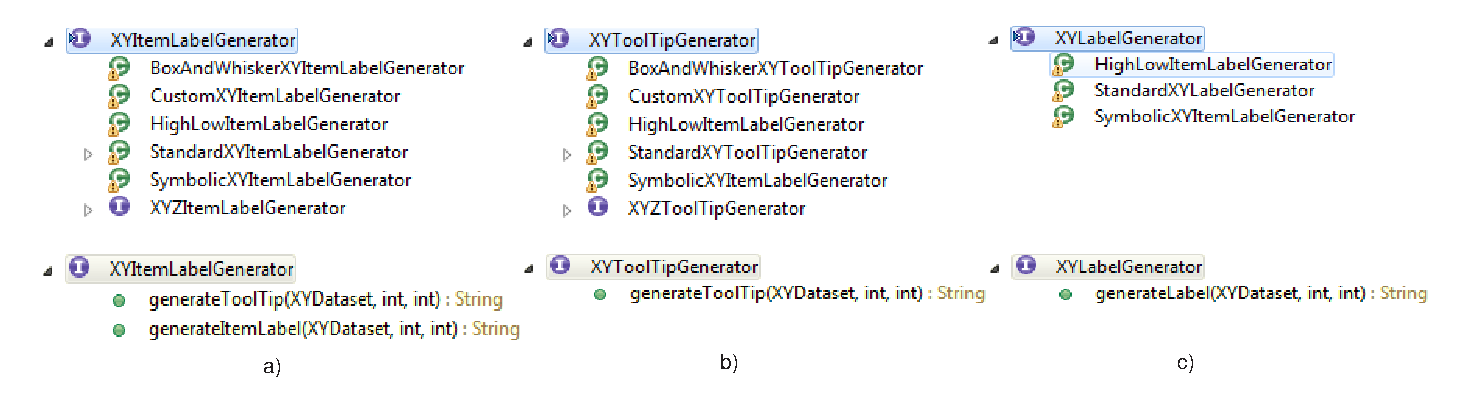
\includegraphics[width=7in]{usage1.eps}}
%\caption{Inheritance and class structure}
%\label{classUsage}
%\end{figure*}
%
%%\begin{figure*}
%%\centerline{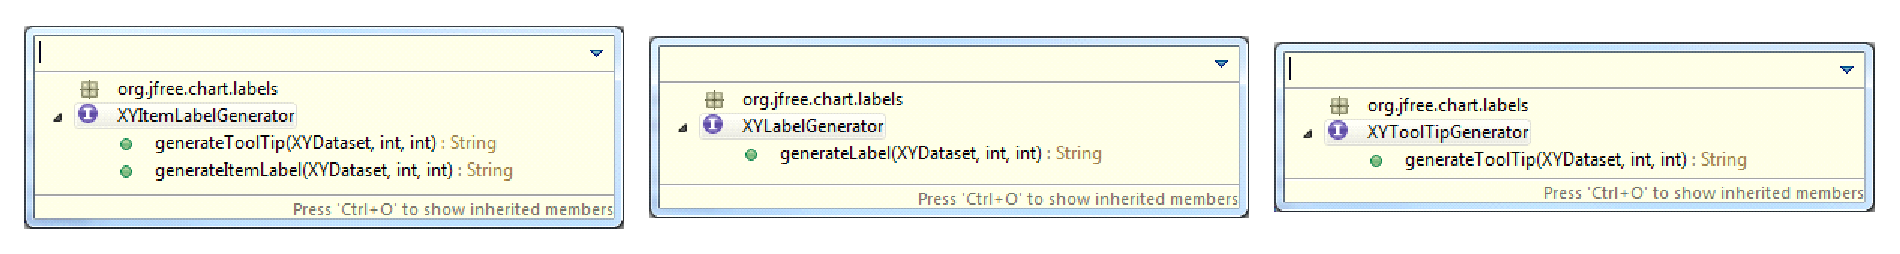
\includegraphics[width=8in]{usage2.eps}}
%%\caption{Class structure}
%%\label{classStruct}
%%\end{figure*}
%
%%\begin{figure*}
%%\centerline{\includegraphics[width=8in]{methodUsage1.eps}}
%%\caption{Method usage}
%%\label{methodUsage1}
%%\end{figure*}
%
%%\begin{figure*}
%%\centerline{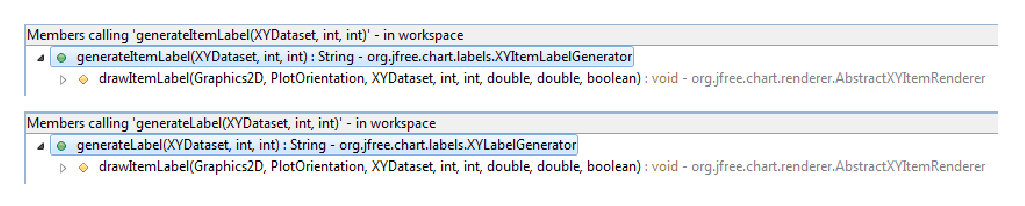
\includegraphics[width=8in]{methodUsage2.eps}}
%%\caption{Method usage}
%%\label{methodUsage2}
%%\end{figure*}
%
%Since graphical charts require textual descriptions, jFreeChart has a
%feature for generating/rendering \emph{labels} and \emph{tooltips} for
%chart items. At version 0.9.17, those two functions of that
%feature are implemented within the interface
%\code{XYItemLabelGenerator} and its descendants, such as
%\code{StandardXYItemLabelGenerator},
%\code{CustomXYItemLabelGenerator}, and
%\code{SymbolicXYItemLabelGenerator}, with two methods
%\code{generateItemLabel} and
%\code{generateToolTip}. Figure~\ref{classUsage}a) illustrates the
%inheritance hierarchy of \code{XYItemLabelGenerator} and its class
%structure.
%
%In version 0.9.17, that feature is realized with two separate class
%hierarchies.
%%those two functions, however, are splitted into two separated class
%%hierarchies.
%The function of \emph{label} generation is implemented in the
%interface \code{XYLabelGenerator} and its descendants, via
%\code{generateLabel} method. The function of \emph{tooltip} generation
%is implemented in the interface \code{XYToolTipGenerator} and its
%descendants, via \code{generateToolTip} method. As shown, during
%evolution, the entities realizing the same feature could be changed in
%their interfaces (e.g. names, locations, parameters) or
%implementations.
%
%Interestingly, the usages of this feature do not change much in the
%system. Moreover, the interactions of the methods/classes of this
%feature with other methods/classes are still quite similar in the
%system. For example, we examined the usages of method
%$A$=\code{XYItemLabelGenerator.generateToolTip} at version 0.9.17 and
%its corresponding method
%$A'$=\code{XYToolTip\-Generator.generateToolTip} at version 0.9.19. We
%saw that $A$ and $A'$ have almost the same set of callers: $A$ has
%sixteen callers and $A'$ has eighteen ones, in which sixteen are the
%same with the ones in $A$ and two are from two newly added
%classes. For two methods \code{XYItemLabelGenerator.generateLabel} and
%\code{XYLabelGenerator.generateLabel}, their callers are exactly the
%same. We also examined the contexts of the calls from those methods to
%other ones in the system and vice versa and found that the contexts of
%such interactions are the same.


%Figure~\ref{methodUsage1}a show the list of callers of
%\code{XYItemLabelGenerator.generateToolTip} within
%jFreeChart. Figure~\ref{methodUsage1}b show the list of callers of
%\code{XYToolTipGenerator.generateToolTip} in the next version. We
%could see that the two lists are the same in two versions. Similarly,
%in Figure~\ref{methodUsage2}, two lists of callers of
%\code{XYItemLabelGenerator.generateLabel} and
%\code{XYLabelGenerator.generateLabel} are also the same.

\subsection{Discussions and Implications}

%Problem statements

As seen in the examples, due to the system's evolution, the program
entities realizing its functionality might be changed in names, source
locations, implementations, or behaviors. A class/method can be {\em
replaced with} or {\em modified into} another one in a new version. If
a developer performs regression testing by running the new version
against existing test cases, (s)he needs to change those existing test
code to fix broken method calls by replacing classes/methods in the
new version. Due to the lack of information, that task could be very
time-consuming. Finding the corresponding entities in the new version
is not straightforward due to the reasons explained earlier.
%Section~\ref{example1sec}.

%%%Moreover, not all existing test cases are required to be adapted.

%If a developer decides to perform regression testing by running the
%new version against existing test cases, (s)he needs to adapt those
%existing test code to use the replacing classes/methods in the new
%version. Due to the lack of documentation, that task is very
%time-consuming with two key challenges. First, finding the
%corresponding entities in the new version is not straightforward due
%to the reasons explained earlier. Second, not all existing test cases
%are required to be adapted.

%If a tester/developer decides to perform regression testing by running
%the new version against existing test cases, (s)he needs to adapt
%those existing test code to use the replacing classes/methods in the
%new version. Due to code evolution and the lack of information, a
%tester often faces two key problems in that task. First, (s)he must
%find by herself/himself those replacements of classes/methods across
%versions. That mapping information is not always available for him/her
%if (s)he is not the author of the source code or if the documentation
%on code changes is not complete. Second, (s)he must go through all
%existing test cases and determine which ones are required to be
%modified in accordance with those replacements. Then, (s)he must
%replace all the references to the old entities with the references to
%the new ones.

This paper addresses the entity tracking problem by introducing
{\tool}, a tool that analyzes two source code versions of a
system and detects the replacements of the classes/methods in which
the entities and their replacements have the same roles in the
system. For example, {\tool} would recommend that
\code{setDragSourceActive} is now replaced by \code{setDragOn}, and
\code{findStackedRangeExtent} is replaced by
\code{getStackedRangeExtent}. {\tool} also identifies the
previous test cases that are required to be repaired in
accordance with those~replacements.

%Therefore, it is desirable to have automated tool support for that
%task during the evolution of the system. A user provides a set of code
%entities of his interest (e.g. classes, methods), and requests the
%tracking tool to detect the replacements/counterparts of those
%entities,   For example, the tool would recommend that the method
%\code{setDragSourceActive} is now replaced by \code{setDragOn}. Such
%recommendation would help him recognize the entities providing the
%functionality of interest in the new version, thus, is useful in
%regression testing tasks.

Developing such an automated tool is challenging because it must take
into account the logical characteristics, such as the dependencies and
interaction of the entities to infer the role similarity in the
system. 
%Tien
%This nature distinguishes the entity tracking problem from that of
%origin analysis, which focuses more on the nature of historical
%existence of entities.
%Tien
%Finding the corresponding entity with the same role via origin
%analysis~\cite{godfrey02,sungkim-wcre05,Kim07} does not always work
%correctly. 
From the view with regard to historical existence, $m$ in jFreeChart
v0.9.20 (Section~\ref{example1sec}) should be mapped to the deprecated
$m$ at v0.9.21. However, {\em repairing existing test cases requires
  $m$ to be mapped to $m'$}. It needs {\em tracking of the entities
  with the same functional role, instead of having the same name or
  location}.

%----------------------------------------------------------------------
The similarity metrics on the entities' names, signatures,
implementation, or callers/callees are applicable. However, an
entity tracking tool cannot solely rely on them because:

1. Entities with the same name might not have the same role, \ie not
  being used in the same way in two versions (see
  Fig.~\ref{example1test}). The names of matched entities might be
  different, \eg due to renaming. Thus, matching entities using only
  the name-based similarity might not always be correct.

2. The callers and/or callees of a method might both be renamed. Thus,
   matching entities solely on the names of their callers/callees
   might be insufficient.

3. The method bodies of matched entities might be quite different
   (Fig.~\ref{drag}). Therefore, using solely code structure-based
   matching would not be sufficient.
%--------------------------------------------------------------------

The functional role of an entity is related to its interaction with
others (\eg how it uses or is used by others). To verify the
interaction/usages of $m$ and $m'$ in jFreeChart v0.9.20 and v0.9.21,
we found that
%all the callers of $m$ were modified to call $m'$.
%Table~\ref{example1} shows that
%Importantly,
they are used in the same set of methods in respective versions. 
%%ASE
%%As seen in Figure~\ref{example1code}, they also call the same
%%ones. 
%%Moreover, the test code is also a method that uses/calls $m$. 
That is, although an entity changes in name or implementation, its
role represented via its \emph{interaction} such as the usage
relations with other entities, is more stable. Thus, the interaction
among code entities can provide useful information for the matching
task. Let us present {\tool}, our novel combination approach of
similarity metrics that also rely on entities' interaction.

%Next, we will present our {\tool} approach.  that provides a novel
% combination of similarity
% measurements based on
% the interactions among entities.


%%%The traditional similarity measurements in original analysis (such as
%%%names, signatures, implementation, callers/callees'
%%%names)~\cite{godfrey02,sungkim-wcre05} are still applicable, however,
%%%an entity tracking tool cannot solely rely on them because:

%%%1. Entities with the same name might not have the same role, i.e. not
%%%  be used in the same way in two versions (see
%%%  Figure~\ref{example1code}). The names of matched entities might be
%%%  different, e.g. due to renaming. Thus, matching entities using only
%%%  the name-based similarity might not always be correct.

%%%2. The callers and/or callees of a method might both be renamed. Thus,
%%%   matching entities solely on the names of their callers/callees
%%%   might be insufficient.

%%%3. The method bodies of matched entities might be quite different
%%%   (Figure~\ref{drag}). Therefore, using solely code structure-based
%%%   matching would not be sufficient.

%In conclusion, the motivating examples suggest the necessity of an
%automated tool for helping developers to tracking entities in evolving
%systems for the purpose of regression testing. Moreover, they suggest
%that such tool cannot solely rely original analysis techniques, but
%should take into account interactions/dependencies among code
%entities. 

\section{Formulation}
\label{model}

\subsection{Key Concepts}

This section presents our model to formulate the tracking problem of
program entities.
%%ASE
%% for adapting regression test cases. 
In our model, a \emph{system} is represented as a set of
{\bf program entities} (\eg classes, methods) with the
{\bf attributes} (\eg name/interface information), and the
%%ASE
%%\emph{relations} and 
{\bf interaction} among those entities (\eg inheritance, invocation,
and collaboration). \emph{Entity tracking} is applied by matching each
entity in the previous version to at most one entity in the next
version. The matching is based on the \emph{similarity} between their
entities. Such similarity is calculated via the weighted sum of the
similarity values of the {\em attributes} and the \emph{interaction}
%%and relations
associated with the entities. 
%
Next, we will describe in detail the key concepts in {\tool}, which
was adapted and extended from the program differencing tool,
iDiff~\cite{ase11-tool}.

%
%entities, attributes, interaction, and the formulation of the matching
%conditions as well as the similarity measurements.

% between entities.

%\subsection{Entity, Attribute, Relation and Interaction}
\subsection{Entity, Attribute, and Interaction}

%Each entity has a set of attribute for signature, inheritance and collaboration attributes for interaction with other entities.

{\tool} is interested in tracking two types of entities: classes
and methods. The attributes
%%ASE
%%relations, 
and interaction of the entities reflect three main kinds of
interaction among entities in a system: method
invocation, data access, and inheritance. {\bf The attributes
and interaction of a class $C$ include}:

\begin{itemize}

\item {\bf Its signature}, containing both the package's and the
  class names. The term \emph{simple name} is used to refer to the
  class name. For example,
  \code{jfreechart.chart.labels.XY\-ItemLabelGenerator} is the
  signature of a class. The corresponding simple name is
  \code{XYItemLabelGenerator};

\item {\bf Inheritance}: $C$ has the attribute
  \code{SuperClass}($C$) to represent a set of classes from which it
  inherits (super-classes), and the attribute \code{SubClass}($C$)
  for the classes/interfaces that inherit/implement $C$ (sub-classes);

\item {\bf Collaboration}: $C$ has the attribute
  \code{Container}($C$) that is the set of classes which declare $C$ as
  a type of their field(s) or have $C$ in their methods'
  signatures. The attribute, \code{Containee}($C$), is the set of
  classes having $C$ as one of their containers, \ie the classes that
  are declared as the types of fields of $C$ or are in one of the
  methods' signatures of $C$. The attribute \code{User}($C$) contains
  the methods that use $C$ in their bodies.

\end{itemize}

\noindent For Java, we consider an interface as an abstract class. {\bf The
attributes and relations/interaction of a method $m$ include}:

\begin{itemize}

\item {\bf Its signature}, containing the package, class, and method's
names, the list of parameter types and the return type. The term {\em
simple name} is used to refer to the combination of class and
method's names in the form of \code{Class.Method}. For example,
\code{DragNDropTool.setDragOn} is the simple name of the method in
Example 2;

%For example here is an signature: \code{long org.jfree.data.xy.XYDatasetTableModel.datasetChanged(long ?org.jfree.data.general.DatasetChangeEvent)} [Tung: please provide a better example]

\item {\bf Inheritance}: $m$ has two attributes of this type.
\code{Overrider}($m$) is the set of methods that override $m$, and
\code{Overridee}($m$) includes the ones that $m$ overrides;

\item {\bf Collaboration}: $m$ has three attributes of
this type. \code{Caller}($m$) contains the methods that call $m$,
while \code{Callee}($m$) is the set of methods that are called within
$m$'s body. \code{Local}($m$) is the set of classes that are used in
the body of $m$ (\ie local types).

\end{itemize}

In {\tool}, the entities, their attributes, relations, and
interaction are represented as an attributed, directed multi-graph,
called {\bf Interaction Graph} (IG) in which

- A node represents a class or a method. The label of each node is the
  corresponding entity's signature;

- Each type of interaction existing between two entities is
  represented as an edge connecting two nodes.

\subsection{Tracking and Similarity}

Each version of the system is represented by an interaction
graph. Entity tracking between two versions aims to match each entity
in one graph of a version to another entity in the other graph of the
later version. 
%Our assumption is that the role of entities and their
%interaction within the system are less likely to change than
%their names or concrete implementations through evolution. 
To track an entity during evolution, we could rely on its role and
interaction with other entities in the system, in addition to names or
implementation. Thus, our matching is mainly based on the similarity
of interaction of the entities, while also takes other measurement
criteria into account to reduce the number of comparisons among
entities.

%enrich the sets of candidates.

\begin{Definition}[{\bf Matched entities}]
An entity $u$ in version 1 is matched to an entity $u'$ in version 2 of the system, denoted by $u \equiv u'$, if their interaction similarity, denoted by $sim(u,u')$, is maximal and is sufficiently large with respect to a pre-defined
threshold, \ie $sim(u,u') \rightarrow max$ and $sim(u,u') \geq
\sigma$.
\end{Definition}

Because an entity from version 1 must be matched to at most one entity
in version 2, {\tool} chooses the matched entities with highest
similarity of interaction. In the case that an entity has the same
interaction similarity with more than one other entities, the
similarity in their names will be used.

\begin{Definition}[{\bf Name similarity}]
The name similarity between two entities, denoted by $nsim(u,u')$, is
measured as the ratio between the length of the longest common
sub-sequence (LCS) and the average length of their simple names.
\end{Definition}

To compute name similarity, {\tool} first breaks two names into
two sequences of tokens based on Hungarian or CamelCase notations,
then applies LCS on two sequences. For example,
$nsim$(\code{setDragSourceActive},\code{setDragOn}) = 2/3.5 = 0.57.

\begin{Definition}[{\bf Interaction similarity}]
The interaction similarity between two entities in two versions is the
weighted sum of the similarity of all of their interaction sets and is
computed~as
$$sim(u,u') = \sum_i{\alpha_i*ssim(I_i(u),I_i(u'))}$$ where
$\alpha_i$s are the non-negative weights such that $\sum_i{\alpha_i} =
1$.
\end{Definition}

In this formula, each set $I_i(u)$ is an {\em interaction set}
of~$u$. It is a set of entities corresponding to one kind of
interaction associated with $u$. Entity $u$ can have multiple
interaction sets. 

If $u$ is a class, its interaction sets include \code{SuperClass}($u$),
\code{SubClass}($u$), \code{Containee}($u$), \code{Container}($u$) and
\code{Users}($u$). If $m$ is a method, its interaction sets include
\code{Caller}($m$), \code{Callee}($m$), \code{Local}($m$),
\code{Overrider}($m$), and \code{Overridee}($m$).  Each of such
interaction for $u$ will be compared with the corresponding
interaction set for $u'$ in the new version. To compare two sets $P$
and $P'$, we define $ssim(P,P')$ as follows:

%is the similarity measurement of two sets $P$ and $P'$, which is
%defined as follows:

\begin{Definition}[{\bf Set similarity}]
The similarity between two sets of entities $P$ and $P'$ is the ratio
between the number of their matched entities and the total number of their
entities:
$$ssim(P,P') = \frac {2*|P \otimes P'|} {|P| + |P'|}$$
\end{Definition}

$P \otimes P'$ denotes the {\em matched subset} of $P$ and $P'$,
covering all matched entities in $P$ and $P'$. Definition~4 means
that $P$ and $P'$ will be more similar if they contain more matched
entities. Formally, the matched subset is defined as

\begin{Definition}[{\bf Matched subset}]
The matched subset of two sets of entities $P$ and $P'$ is the list of pairs of their matched entities, i.e. $P \otimes P' = \{(u \in P, u' \in P') |u \equiv u\}$.
\end{Definition}

%The intuition of this definition is that, the larger the number of
%common entities between $P$ and $P'$ is, the more they are
%similar. Conventional wisdom would choose the set of common entities
%as the intersection set of $P$ and $P'$. However, $P$ and $P'$ are
%sets of entities between two versions, which might have changed
%entities. Therefore, to {\em take the changes of entities into
%consideration}, we define the {\em common entities of $P$ and $P'$} as
%the following

Let us take Fig.~\ref{drag} to show an example of the similarity
between two sets of $I$=\code{Callers}(\code{setDragSourceActive}) and
$I'$=\code{Callers}(\code{setDragOn}). Assume that, we could match
\code{active} to \code{active}, and \code{deactivate} to
\code{deactivate} in two versions of class \code{DragNDropTool}, then
their matched subset contains those two pairs, $ssim(I,I')$=
(2*2)/(2+2) = 1.0.

%Assuming that at the time of computing for these two sets, {\tool}
%already had the mapping between the classes that have same names, then
%$ssim(I_1,I_2)=2/6=0.33$.
%Now given that more matchings are found between the classes whose
%names contain \code{ItemLabel} and \code{ToolTip}, then
%$ssim(I_1,I_2)$ could reach 1.0.

%%%This matching problem is really the problem of finding maximum
%%%cardinality bipartite matching of $P$ and $P'$, using $sim(u,u') \geq
%%%\sigma$ as a condition to make the edges.

%To avoid recursive computation, we develop an approximate, iterative algorithm, which will be explained next.

%- A system is represented as an attributed, interaction/dependency graph:
%
%+ Each node represents an entity in the system: package, class/interface, method.
%
%+ A node has a set of attributes: interface (pathname/signature), implementation (body usage vector).
%
%+ Edges represent different relations between nodes: interaction/dependency caller-callee (client-server) - employer-employee/co-operate/collaborator, colleague
%
%X and Y are employer-employee related: Y is used in X, used = inherited, called, declared as field/variable/parameter.
%
%X and Y are colleague related: are both used inside Z' implementation.
%
%Philosophy/Assumption: evolved entities might have changes in interface or implementation but little in interaction. Especially interaction is the most stable (changes at design level).
%
%Thus, similarity on interface/implementation/interaction of entities could be used to tracking them.
%
%Define: sim(x,y) = total similarity
%
%        or matched(x,y) = some conditions...
%
%Problem: graph matching, maximize number of matches.
%
%\subsection{Similarity measurement}
%
%This section discusses the similarity measurements designed for different types of software entities (package, class, method).
%
%1. Method similarity
%
%- signature: return type + name + list of parameter types
%
%- internal interactions:  usages of other methods within its implementation
%
%- external interations: its usage within other methods' implementations
%
%- local types: usages of classes within its implementation
%
%2. Class similarity
%
%- signature: name
%
%- inheritance/interface relation
%
%- declared classes
%
%- body: synthesized from all normalized contained methods' features. All methods' vectors are normalized to have the length of 1 and summed up.
%
%3. Package similarity
%
%- signature: name and containg package's name
%
%- body: all contained packages and classes
%
%4. Name similarity measurement: Names are tokenized based on naming convention and then compared using long common sub-sequence
%
%5. Structure vector similarity: ratio between shared structural features (including the frequency) and total structural features.
%
%6. Interaction set/vector similarity: set similarity: $$sim(X,Y) = \frac {|X \cap Y|} {|X \cup Y|} $$, or distance (normalized, or Spearman correlation??? )???

\section{{\tool} Algorithms}
\label{algosection}

In this section, we present the key algorithms in {\tool}.
%%ASE
%%to solve the problem formulated in Section~\ref{model}.
The main algorithm (\code{System\-Match}) is for matching the program
entities between two versions of a system, using Definition~1 and
Definition 3 for the matching criteria. This algorithm utilizes a
greedy algorithm (\code{Simple\-Match}) to match the entities in two
given sets. The last algorithm, \code{FindTestCase}, uses the list of
matched entities to find existing test cases that need~fixing.

%We first start with the algorithm to calculate
%the common subset of two sets of entities as in Definition 5, which
%can be used to detect the matching between the entities in any two
%sets. Then, we present our algorithm to match the entities between two
%versions of the system for feature tracking.

% which selects the
% candidates and calculates the common subset via the first algorithm.

%The pseudo-code for algorithms is in Figure~\ref{matching}.

\subsection{Key Design Ideas}

Initially, one might think that matching the entities could be done
using a classical bipartite matching algorithm following
Definition~1. However, such a (brute-force) algorithm will not work
because of the following issues:

1. {\em Efficiency}. Classical bipartite matching has the
   computational complexity of $O(n^3)$, with $n$ being the number of
   entities. With this high level of computational complexity, the
   algorithm does not scale well for large systems with several
   thousands of entities (classes and methods).

2. {\em Determinism}. The criteria for matched entities is recursive
   by nature. Assume that $u$ and $v$ are two related entities. To
   match $u$ to $u'$ (Definition~1), we might need to compute the
   similarity of two sets including $v$ and some entity $v'$ related
   to $u'$ (Definitions~3 and 4). This computation requires the
   matching information of $v$ to $v'$ (Definition~5). If $v$ and $v'$
   are not yet matched, this matching computation in turn requires the
   matching of $u$ and $u'$, which is currently under calculation.


%uses the knowledge from already-matched code entities to incrementally
%update the similarities of not-yet-matched entities for further
%matching.

To overcome these two issues, we have designed a novel algorithm for
this matching problem. The algorithm works in an {\bf iterative}
fashion, using \emph{already-matched} entities to find new candidates
and compute their similarity for further matching. That is, instead of
considering all pairs of entities as possible matched pairs, {\tool}
maintains and processes a list of pairs as candidates. To compute the
similarity of two entities in a candidate pair, {\tool} uses only the
already-matched entities (\eg in finding the common subset in
Definition~5), disregarding the recursive nature of the similarity
calculation. If they are matched, their related entities
(\eg methods, callers, callees, or sub-classes) are potentially
matched entities, thus, are considered to be added to the list of
candidates (via re-calculating their similarity). All the remaining
entities are compared pairwise at the final step, which is much less
expensive than the pairwise comparison at the beginning.

At first, {\tool} uses name-based and implementation-based criteria to
find the initial candidates. That is, it initializes its candidate
list with the entities having the same simple names (class or
method names without the signatures), and then the entities with
similar bodies. To find the entities having similar bodies, {\tool}
utilizes locality-sensitive hashing (LSH)~\cite{lsh} on the
characteristic vectors extracted from their implementation code. For
example, the body vector of a class is a binary vector of the
occurrences of classes used in its fields and
methods. Locality-sensitive hashing is a hashing scheme that provides
the same hash code for similar vectors. Thus, to find entities with
similar implementation code, {\tool} hashes their vectors and only
compares the entities having the same hash code.

Next, we will discuss the details of three algorithms to find the
matched subset of two entity sets (Definition 5), to match the
entities between two versions (Definition 1), and to detect the test
cases that need adaptation.

\subsection{Simple Matching}
\label{simplematch}

\begin{figure}
\begin{lstlisting}[stepnumber=1,numbers=left,numbersep=-5pt]
		function match($U$, $U'$, $N$)
		//find matched set $U \otimes U'$, output as a map $N$
			$N$.clear()
			repeat
				$L$ = new descendingly sorted list associating with $sim$
				for all $(u,u') \in U \times U'$
					if($sim(u,u') \geq \sigma$)
						$L$.add$(u,u')$ //collect all pairs of candidates
				if $L = \emptyset$ break //no pair collected => done
		
				while($L \neq \emptyset$)
					$(u,u') = L$.top() //match top ones
					$N$.add$(u,u')$
					remove all $(u,v') \in L$ and $(v,u') \in L$ //remove their pairs
			until false
\end{lstlisting}
\caption{Simple Matching Algorithm}
\label{cmatching}
\end{figure}

Let us first describe the algorithm to match the entities between two
sets of entities $U$ and $U'$ in two different versions
(Definition~5). It is called \code{simple match}, because it
is a separate computation step for
%simplifies the computation of
the similarity of two entities without recursion. That is, for each $u
\in U$ and $u' \in U'$, if $u$ and $u'$ are already matched, then
$sim(u,u') = 1$. Otherwise, it initializes $sim(u,u')=nsim(u,u')$ with
$nsim$ being their name similarity defined in Definition 2 and updates
this value if more information is available. Thus, $sim$ is always
defined for any pair of entities $u$ and $u'$. In addition, it uses a
greedy approach that iteratively selects the matching pairs
descendingly by their similarity degrees.

%, thus, reducing the complexity to $O(n^2)$.

Fig.~\ref{cmatching} illustrates the algorithm. First, it
collects all pairs of entities $u \in U$ and $u' \in U'$ satisfying
the necessary condition for matching, \ie$sim(u,u') \ge
\sigma$. Those pairs are maintained in a heap, \ie a descending
sorted list $L$ (lines 5-8), sorted by the similarity
$sim(u,u')$. Then, {\tool} repeatedly detects the pair $(u,u')$ with
the highest $isim$ in that sorted list as a matched pair (lines
12-13), and removes all pairs containing either one of its two
entities $u$ or $u'$ (line 14). This step ensures that each entity $u$
is matched at most one other entity $u'$ in which the interaction
similarity $isim$ is maximal. The newly matched pairs now are used
to recalculate $sim$ for the non-matched entities in $U$ and $U'$
when the process repeats (lines 4-15) until no other candidates
can be collected (line 9).

%This greedy approach is reasonable in this situation because we want to map each entity in one version with at most one entity in the other version of the system and there are no two entities having the same signature in one version of a system.

\subsection{System Matching}


Fig.~\ref{matching} illustrates the main algorithm to match entities
from a version $P$ to a new version $P'$. It outputs a map $C$
containing pairs of matched classes $(c,c')$ and a map $M$ containing
pairs of matched methods $(m,m')$. This algorithm has two main steps:
matching the classes and then the methods. For those steps, the same
procedure is applied: first, it processes for the
candidates with the same simple name, then for the candidates having
similar characteristic vectors extracted from body code, and finally,
all remaining candidates are compared pair-wise. The candidates with the
same names or similar vectors are identified via LSH.

\begin{figure}
\begin{lstlisting}[stepnumber=1,numbers=left,numbersep=-5pt]
		function track($P, P'$)
		//match entities in two versions $P$ and $P'$ to two maps $C$ and $M$
			$C$ = matchClasses()
			$M$ = matchMethods()
		return $C, M$
		
		function matchClasses()
			$X$.addAll(classes of $P$) and $X'$.addAll(classes of $P'$)
			$N$ = HashbyName($X$) and $N'$ = HashbyName($X'$)
			for each $n$ in $N$.keys $\cap$ $N'$.keys: process($N(n), N'(n), C$)
			$H$ = LSHbyBodyVector($X$) and $H'$ = LSHbyBodyVector($X'$)
			for each $k$ in $H$.keys $\cap$ $H'$.keys: process($H(k), H'(k), C$)
			process($X, X', C$)
		return $C$
		
		function matchMethods()
			$X$.addAll(methods of $P$) and $X'$.addAll(methods of $P'$)
			for each matched classes pair $(c,c') \in C$:
				process($c$.methods, $c'$.methods, $M$)
			$N$ = HashbyName($X$) and $N'$ = HashbyName($X'$)
			for each $n$ in $N$.keys $\cap$ $N'$.keys: process($N(n), N'(n), M$)
			$H$ = LSHbyBodyVector($S$) and $H'$ = LSHbyBodyVector($S'$)
			for each $k$ in $H$.keys $\cap$ $H'$.keys: process($H(k), H'(k), M$)
			process($X, X', M$)
		return $M$
		
		function process($U, U', O$)
		//match entities in $U$ and $U'$, add them to the map of matched entities $O$, and remove them from the remaining sets.
			match($U$, $U'$, $N$)
			$O$.addAll($N$)
			$X$.removeAll($N$.keys)
			$X'$.removeAll($N$.values)
\end{lstlisting}
\caption{System Matching Algorithm}
\label{matching}
\end{figure}

\subsubsection{Matching Classes}

{\tool} matches the classes (lines 7-14) before matching the methods
(lines 16-25). To match classes, it first processes the candidates
having the same simple names (lines 9-10). It uses string-based
hashing scheme to hash the classes into buckets, each bucket is a
set of entities having the same name. Then, for each pair of buckets
for the same name, it uses \code{simple match}
(Section~\ref{simplematch}) to match their entities. The matched
entities are added to the global map $C$ and removed from the sets of
remaining entities $X$ and $X'$.

Then, {\tool} processes the candidates having sufficiently similar
vectors extracted from their bodies (lines 11-12). The process is
similar to the previous step. The vector extracted from a class $c$
describes the classes used in $c$. Instead of string-based hashing,
{\tool} uses locality-sensitive hashing to hash and find similar
vectors. Finally, {\tool} matches the remaining classes pairwise (line
13).

Note that, the similarity of names or body code is used only to
suggest the candidates for matching. Those candidates are actually
matched using the interaction similarity (defined in Definition~3) as
in the algorithm in Section~\ref{simplematch}.

\subsubsection{Matching Methods}

To match the methods, the algorithm first finds the candidate methods
in the classes that are matched in the previous step (lines 18-19)
because if the classes are matched, their methods should be the
candidates for matching. However, there are many cases in which the
methods might be extracted/split from the old class. Thus, the next
step of the algorithm is to find the candidate methods {\em across the
classes}. Once again, {\tool} uses name and body to suggest the
candidates. It starts processing the candidate methods in any classes
having the same names (lines 20-21). Then, it considers the methods
having similar bodies (lines 22-23). The body vector of a method is a
binary vector of the occurrences of methods that are called in its
body, \ie the vector representing the set \code{Callee}. Finally, the
remaining methods are pairwise compared (line 24). Similar to the
classes, candidate methods are matched using the algorithm in
Section~\ref{simplematch} with the interaction similarity criteria in
Definition~1.

%\begin{figure}
%\begin{lstlisting}[basicstyle=\small\sffamily, stepnumber=1,numbers=left, language = Delphi]
%function FeatureTrack($P, P'$)
%// Match entities in two versions $P$ and $P'$ to a map $M$
%//  Step 1.1. Match classes using name for candidates
% $C$.addAll(classes of $P$) and $C'$.addAll(classes of $P'$)
% $H$ = HashbyName($C$) and $H'$ = HashbyName($C'$)
% for each name $n$ in $H$.keys $\cap$ $H'$.keys //candidates by name
%  match($H(n), H'(n), N$) and update($N, M_C, C, C'$)
%
%//  Step 1.2. Match classes using body for candidates
%//  use locality-sensitive hashing: similar body => same hash code
% $H$ = LSHbyBodyVector($C$) and $H'$ = LSHbyBodyVector($C'$)
% for each hash code $k$ in $H$.keys $\cap$ $H'$.keys
%  match($H(k), H'(k), N$) and update($N, M_C, C, C'$)
%
%//   Step 1.3. Match all remaining classess
% match($C, C', N$) and update($N, M_C, C, C'$)
%
%//  Step 2.1. Match methods using name for candidates
% $M$.addAll(methods of $P$) and $M'$.addAll(methods of $P'$)
% for each matched classes pair $(A,A') \in M_C$
%  match($A$.methods, $A'$.methods, $N$) and update($N, M_M, M, M'$)
% $H$ = HashbyName($M$) and $H'$ = HashbyName($M'$)
% for each name $n$ in $H$.keys $\cap$ $H'$.keys //candidates by name
%  match($H(n), H'(n), N$) and update($N, M_M, M, M'$)
%
%//  Step 2.2. Match methods using body for candidates
% $H$ = LSHbyBodyVector($M$) and $H'$ = LSHbyBodyVector($M'$)
% for each hash code $k$ in $H$.keys $\cap$ $H'$.keys
%  match($H(k), H'(k), N$) and update($N, M_M, M, M'$)
%
%//  Step 2.3. Match all remaining methods
% match($M, M', N$) and update($N, M_M, M, M'$)
%
%function update($N, O, U, U'$)
%//remove newly-found matched entities $N$ from unmatched entities $U$ and $U'$ and add them to global matched entities $O$
% $O$.addAll($N$)
% $U$.removeAll($N$.keys)
% $U'$.removeAll($N$.values)
%
%\end{lstlisting}
%\caption{Entities Matching Algorithm}
%\label{matching}
%\end{figure}

\subsection{Recommending Repairing Broken Method Calls}
{\tool} uses a simple criterion to find the previously run test cases
that require an repair. That is, a test case $t$ is recommended for repair if it uses an entity $u$ (\eg declares an object of class $u$ or calls method $u$) that needs to be replaced. {\tool} considers $u$
to be replaced if:

1. It is not matched to any entity in the new version (\ie is deleted), or

2. Its matched entity $u'$ has a different signature.

Using this criteria, after matching all entities for the system,
{\tool} analyzes all the existing test cases. If a test case
$t$ satisfies the aforementioned criterion with some entities $u$, {\tool} will output $t$, $u$, and its matched entity $u'$ (if any) as the recommendation, \ie $t$ is recommended for repair in which $u$ is replaced by $u'$.

%(In the future works, we plan to use more sophisticated change
%analysis techniques to find the test cases that is affected by the
%change of the system). 

\section{Empirical Evaluation}

This section discusses the empirical evaluation of {\tool} on
real-world subject systems. All experiments were carried out on a
computer with CPU Intel Core 2 Duo T7500 2.2 GHz, 3GB RAM. For the
parameters in experiments, we set the threshold on interaction
similarity $\sigma = 0.75$ (in Definition 1) and use an evenly weighted
sum in computing the total interaction similarity (in Definition 3).

\subsection{Benchmark Dataset}
To evaluate the quality of entity tracking and test case repair
recommendation in {\tool}, we build a benchmark dataset from two
open-source systems with four pairs of releases. For each pair $v_1$
and $v_2$ under analysis, we find all test cases that exist in $v_1$
and are repaired in $v_2$ (such as in
Fig.~\ref{example1test}). For a test case and its repaired copy in
the new version, we manually match the entities with the same
functional role in the respective test code. If $m$ is paired with a
different entity $m'$ (such as two methods
\code{DataUtilities.getStackedRangeExtent} and
\code{DataUtilities.findStackedRangeExtent}), we consider this pair as
a replaced pair (R), and mark the test case to have a replacement
operation. Otherwise, the pair is marked as an unchanged pair (U), such as
two methods \code{Range.getLowerBound} and \code{Range.getLowerBound}.

% ------- Special case --------
When an entity in a test case cannot be matched in the repaired test
case, it is considered as deleted and is paired with
\code{null}. Because {\tool}'s goal is to detect one-to-one
replacements, we do not consider the cases in which the role of an
entity is replaced with that of multiple entities, or vice versa, in
the new version. We also discard any removed test cases and any
changed parts in test cases that are un-related to the replacements of
existing program entities, \eg updating the values in assertion
expressions, deleting redundant code, or adding new code. We consider
matched pairs of the entities used in unchanged test cases as the
unchanged pairs. Finally, for each existing test case in $v_1$ and its
repaired/unchanged version in $v_2$, we have a list of matched pairs of
entities, with corresponding operations: replacement (R) or unchanged
(U). Table~\ref{matches} shows such a list for the example in
Fig.~\ref{example1test}. The utility methods for testing
(\eg \code{assertEquals}) are discarded.

\begin{table}
%\footnotesize
%\footnotesize
\small
\caption{Matched Entities of Test Cases in Fig.~\ref{example1test}}
%\setlength{\tabcolsep}{2pt}
% Table generated by Excel2LaTeX from sheet 'Sheet2'
\begin{tabular}{llr}
\addlinespace
\toprule
Old Entity & New Entity & Op. \\
\midrule
DataUtilities.getStacked... & DataUtilities.findStacked... & R \\
CategoryDataset & CategoryDataset & U \\
Range.getLowerBound & Range.getLowerBound & U \\
Range.getUpperBound & Range.getUpperBound & U \\
\bottomrule
\end{tabular}%
\label{matches}
\end{table}


\begin{table}[t]
%[htbp]
%\scriptsize
\small
  \centering
  \caption{Benchmark Dataset}
  \setlength{\tabcolsep}{2.5pt}
	\begin{tabular}{l|l|rr|rrr}
    \addlinespace
    \toprule
    Systems & Version Pairs & \multicolumn{2}{c|}{Test Cases} & \multicolumn{3}{c}{Matched Pairs} \\
    \midrule
      &       & Chged & No & Chged & No & Null \\
    \hline
JFreeChart & 0.9.8 (1) - 0.9.9 (2) & 53    & 144   & 41    & 190   & 4 \\
      &  0.9.18 (3) - 0.9.19 (4) & 26    & 486   & 64    & 716   & 2 \\
JTopas & 0.6 (1) - 0.7 (2) & 6     & 53    & 8     & 191   & 7 \\
      & 0.7 (2) - 0.8 (3) & 56    & 12    & 22    & 87    & 9 \\
\midrule
Total &       & 141   & 695   & 135   & 1184  & 22 \\
\bottomrule
    \end{tabular}%
  \label{tab:dataset}
\end{table}

%We also process the unchanged test cases and consider all pairs of the
%entities used in those test cases as the unchanged pairs.  There are
%test cases in which an entity in the original test case is actually
%deleted or has its role replaced by multiple entities in the adapted
%test case (or vice versa). Because these cases are beyond the scope of
%{\tool}, we consider that entity is matched to \code{null}. We count
%only once for the repeated pairs of matched entities in our benchmark.

Table~\ref{tab:dataset} shows the data collected in this benchmark
dataset. The largest collected data comes from the version pair 0.9.18
and 0.9.19 of JFreeChart, which contains 26 repaired test cases,
and 486 unchanged test cases. From those test cases, we extracted 64
replaced and 716 unchanged pairs. The entire dataset has 141
repaired test cases, and 1,319 matched entity pairs with 135 replaced,
and 1,184 unchanged pairs. There are totally 22 deleted entities (\code{null}
pairs) in those test cases.

\subsection{Accuracy of Entity Matching}
\label{acc}

To evaluate the accuracy of {\tool} in entity matching, we conducted
an experiment by running {\tool} on each pair of versions in our
benchmark dataset in comparison with the state-of-the-art entity tracking
tool from Kim, Pan, and Whitehead
(KPW)~\cite{sungkim-wcre05}. Each tool reports the matches for all
possible entities in the subject systems, however, we evaluate the
matching accuracy for only the entities in the test cases
(\code{Test}) for which the correct matching information is available
in the benchmark. A reported pair is considered as correct if it is in
the benchmark. Accuracy is measured as the ratio between the number of
correctly reported pairs (column \code{Corr.}, Table~\ref{tab:compare}) and
the number of all matched pairs in the benchmark.

% (which need to be reported).

%\begin{table*}[t]
%\scriptsize
%  \centering
%  \caption{Sensitivity Analysis}
%\begin{tabular}{lrrrrrrrr}
%\addlinespace
%\toprule
%W/o   & \multicolumn{4}{c}{JFreeChart 0.9.8 - 0.9.9} & \multicolumn{4}{c}{JTopas 0.6 - 0.7} \\
%\midrule
%      & Test  & Corr. & Acc.  & T(s)  & Test  & Corr. & Acc.  & T(s) \\
%Name  & 243   &       &       &       & 206   &       &       &  \\
%Clone & 243   &       &       &       & 206   &       &       &  \\
%Caller & 243   &       &       &       & 206   &       &       &  \\
%Callee & 243   &       &       &       & 206   &       &       &  \\
%Local & 243   &       &       &       & 206   &       &       &  \\
%Overrider & 243   &       &       &       & 206   &       &       &  \\
%Overridee & 243   &       &       &       & 206   &       &       &  \\
%None  & 243   & 228   & 94\%  & 240  & 206   & 204   & 99\%  & 5 \\
%\bottomrule
%\end{tabular}%
%  \label{tab:sen}%
%\end{table*}%


\begin{table*}[htbp]
%\scriptsize
  \centering
  \caption{Comparison of Entity Matching Accuracy}

%\begin{tabular}{llrrrrrrrrrr}
%    \addlinespace
%    \toprule
%    System & Version Pair & \multicolumn{3}{c}{Entities} & \multicolumn{3}{c}{iTrack} & \multicolumn{3}{c}{KPW} & \multicolumn{1}{c}{$\bigcap$} \\
%    \midrule
%      &       & Class & Method & In Test & Correct & Acc.  & Time  & Correct & Acc.  & Time  &  \\
%JFreeChart & 0.9.8(1) - 0.9.9(2) & 571-593 & 4132-4497 & 231   & 217   & 94\%  & 5min  & 191   & 83\%  & 30min & 191 \\
%      & 0.9.18(3) - 0.9.19(4) & 783-821 & 6867-7143 & 780   & 746   & 96\%  & 3min  & 719   & 92\%  & 15min & 719 \\
%JTopas & 0.6(1) - 0.7(2) & 77-81 & 887-939 & 199   & 199   & 100\% & 12s    & 199   & 100\% & 22s   & 199 \\
%      & 0.7(2) - 0.8(3) & 81-76 & 939-771 & 109   & 103   & 94\%  & 21s   & 88    & 81\%  & 470s  & 88 \\
%\midrule
%Average &       &       &       &       &       & 96\%  &       &       & 89\%  &       &  \\
%\bottomrule
%    \end{tabular}%

% Table generated by Excel2LaTeX from sheet 'Sheet1'
\setlength{\tabcolsep}{4pt}
\begin{tabular}{lr|rrr|rrr|rrr|r|rrr|rrr}
\addlinespace
\toprule
System & Versions & \multicolumn{3}{c|}{Entities} & \multicolumn{3}{c|}{iTrack} & \multicolumn{3}{c|}{KPW} & \multicolumn{1}{c|}{$\bigcap$} & \multicolumn{3}{c|}{iTrack w/o Name} & \multicolumn{3}{c}{iTrack w/o Clone} \\
\midrule
      &       & Class & Method & Test  & Corr. & Acc.  & Time  & Corr. & Acc.  & Time  &       & Corr. & Acc.  & Time  & Corr. & Acc.  & Time \\
JFreeChart & (1) - (2) & 571-593 & 4132-4497 & 231   & 217   & 94\%  & 4m14s & 191   & 83\%  & 30min & 191   & 214   & 93\%  & 8m15s & 219   & 95\%  & 4m50s \\
      & (3) - (4) & 783-821 & 6867-7143 & 780   & 746   & 96\%  & 2m32s & 719   & 92\%  & 15min & 719   & 744   & 95\%  & 5m34s & 743   & 95\%  & 2m57s \\
JTopas & (1) - (2) & 77-81 & 887-939 & 199   & 199   & 100\% & 9s    & 199   & 100\% & 22s   & 199   & 199   & 100\% & 10s   & 199   & 100\% & 9s \\
      & (2) - (3) & 81-76 & 939-771 & 109   & 103   & 94\%  & 24s   & 88    & 81\%  & 470s  & 88    & 92    & 84\%  & 32s   & 102   & 94\%  & 27s \\
\midrule
Average &       &       &       &       &       & 96\%  &       &       & 89\%  &       &       &       & 93\%  &       &       & 96\%  &  \\
\bottomrule
\end{tabular}%
  \label{tab:compare}%
\end{table*}%

%Table~\ref{tab:compare} shows the result.

Columns \code{Acc.} in Table~\ref{tab:compare} show the accuracy
of both tools. In most cases, {\tool} has accuracy of more than
90\%, and is always higher than that of KPW for all subject
systems. Interestingly, {\tool} reports more correctly matched pairs
than KPW and its correctly detected pairs cover KPW's result (column
\code{$\bigcap$}). We also found that KPW misses the
cases in which methods are replaced with the new ones having different
implementations and names, and even their callers/callees in some
cases are renamed (as in the motivating examples). This result shows
that {\tool} is better suited for entity tracking in test cases.
%matching and for repairing existing test cases.
%This result shows that {\tool} is highly correct in tracking entities
%for test case adaptation in regression testing, and it is better than
%KPW in this task. This result is expected because as explained in
%Section~\ref{empi}, {\tool} is better suited for this task than origin
%analysis approaches.
Let us discuss a few
%interesting
cases from our experiments.

%, which illustrate how our tool is better suited???

%----------------------------------------------------------------
%%%\subsubsection{Pie Dataset Total Computing}

%%%When rendering pie charts, jFreeChart needs to calculate the ratio of
%%%each pie to the whole chart. To do that, jFreeChart first calculates
%%%the total of all values of the given a dataset for the pie chart under
%%%rendering. At version 0.9.18, this function is provided by method
%%%\code{DatasetUtilities.get\-PieDatasetTotal}. At version 0.9.19, this
%%%method is modified into
%%%\code{DatasetUtilities.calculatePieDatasetTotal}.  {\tool} is also
%%%able to match those two methods while KPW's tool cannot.
%----------------------------------------------------------------

\vspace{0.04in} {\bf Supporting Multiple Datasets in jFreeChart.}
\code{XYPlot} is the class in jFreeChart that supports plotting charts
for X-Y curves. To support plotting multiple datasets in the same
chart, before version 0.9.19, \code{XYPlot} distinguishes
\emph{primary} and \emph{secondary} datasets, and uses two different
sets of methods for each kind. For example,
%method \code{getDataset} is used to get the primary dataset and
method \code{getDomainAxis} is used
to get a \code{ValueAxis} for the primary dataset while
%method \code{getSecondaryDataset}is used to get a secondary dataset  or
method \code{getSecondaryDomainAxis} is used to get a \code{ValueAxis} for the secondary dataset indexed by its parameter.

However, at version 0.9.19, this class has a change to \emph{``removed
major distinction between primary and secondary datasets, renderers
and axes''}. Since the implementation of methods supporting secondary
datasets is more general and applicable for the primary
dataset, all methods that were used to support the primary dataset are
now removed, and all methods that were used to support secondary
datasets are now changed to support both primary and secondary
datasets. Thus, those methods are renamed and modified, with the word
``Secondary'' removed. Fig.~\ref{plot} illustrates the source code
of the methods \code{getDomainAxis} and \code{getSecondaryDomainAxis}
in two versions. {\tool} was able to match all methods supporting
secondary datasets in 0.9.18 to the corresponding methods in 0.9.19
while KPW incorrectly matched the two methods \code{getDomainAxis} in two versions to
each other.

\begin{figure}[t]
XYPlot.java in version 0.9.18
\begin{lstlisting}[language = Java]
public ValueAxis getDomainAxis() {
	ValueAxis result = this.domainAxis;
	if (result == null) {
		Plot parent = getParent();
		if (parent instanceof XYPlot) {
			XYPlot xy = (XYPlot) parent;
			result = xy.getDomainAxis();
	.........
public ValueAxis getSecondaryDomainAxis(int index) {
	ValueAxis result = null;
	if (index < this.secondaryDomainAxes.size()) {
		result = (ValueAxis) this.secondaryDomainAxes.get(index);
	}
	if (result == null) {
		Plot parent = getParent();
		if (parent instanceof XYPlot) {
			XYPlot xy = (XYPlot) parent;
			result = xy.getSecondaryDomainAxis(index);
		}
	}
	return result;
}
\end{lstlisting}
XYPlot.java in version 0.9.19
\begin{lstlisting}[language = Java]
public ValueAxis getDomainAxis(int index) {
	ValueAxis result = null;
	if (index < this.domainAxes.size()) {
		result = (ValueAxis) this.domainAxes.get(index);
	}
	if (result == null) {
		Plot parent = getParent();
		if (parent instanceof XYPlot) {
			XYPlot xy = (XYPlot) parent;
			result = xy.getDomainAxis(index);
		}
	}
	return result;
}
\end{lstlisting}
%\caption{Getting Domain Axis in JFreeChart}
\caption{The mapped Methods have different Names and Implementations}
\label{plot}
\end{figure}

\vspace{0.03in} {\bf Adding Auto-Pruning Functionality.} In JFreeChart
from version 0.9.16 to 0.9.17, the constructor $m_1$ =
\code{DefaultTableXYDataset(XYSeries)} was deprecated and a new
constructor $m_2$ = \code{DefaultTableXYDataset(boolean)} was
introduced to add the functionality of auto-pruning
(Fig.~\ref{autoprun}). Since $m_2$ has different parameter type and
much different body from $m_1$, KPW cannot match them together, while
{\tool} can.

% even if $m_1$ is deleted in the new version.

\begin{figure}[t]
DefaultTableXYDataset.java in version 0.9.16
\begin{lstlisting}[language = Java]
public DefaultTableXYDataset(XYSeries series) {
	this.data = new ArrayList();
	this.xPoints = new HashSet();
	if (series != null) {
		if (series.getAllowDuplicateXValues()) {
			throw new IllegalArgumentException("...");
		}
		updateXPoints(series);
		data.add(series);
		series.addChangeListener(this);
	}
}
\end{lstlisting}
DefaultTableXYDataset.java in version 0.9.17
\begin{lstlisting}[language = Java]
public DefaultTableXYDataset(boolean autoPrune) {
	this.autoPrune = autoPrune;
	this.data = new ArrayList();
	this.xPoints = new HashSet();
}
\end{lstlisting}
%\caption{Adding Auto-Pruning in JFreeChart}
\caption{The Mapped Methods have different Parameters and Implementations}
\label{autoprun}
\end{figure}

%@Deprecated
%public DefaultTableXYDataset(XYSeries series) {
% this.data = new ArrayList();
% this.xPoints = new HashSet();
% if (series != null) {
%  if (series.getAllowDuplicateXValues()) {
%   throw new IllegalArgumentException("...");
%  }
%  updateXPoints(series);
%  this.data.add(series);
%  series.addChangeListener(this);
%}
% this.autoPrune = false;
%}

\subsection{Accuracy on Recommending Repairs in Test Cases}

\begin{table}[t]
\small
  \centering
  \caption{Test Case Repairing Recommendation Accuracy}
  \setlength{\tabcolsep}{3pt}
	\begin{tabular}{lr|rrrr|rrr}
    \addlinespace
    \toprule
    System & Vers. & \multicolumn{4}{c|}{Test Cases Rec.} & \multicolumn{3}{c}{Replacement Rec.} \\
    \midrule
      &       & Rec.  & Corr. & Acc.  & Miss  & Rec.  & Corr. & Acc. \\
    \hline
JFreeChart & (1) - (2) & 52    & 52    & 100\% & 1     & 489   & 471   & 96\% \\
      & (3) - (4) & 26    & 26    & 100\% & 0     & 1653  & 1613  & 98\% \\
JTopas & (1) - (2) & 6     & 6     & 100\% & 0     & 581   & 579   & 99\% \\
      & (2) - (3) & 55    & 55    & 100\% & 1     & 422   & 355   & 84\% \\
\bottomrule
    \end{tabular}%
  \label{tab:recom}%
\end{table}%

To evaluate the correctness of repair recommendation in {\tool},
we conducted another experiment. We ran {\tool} on each pair of
releases in our benchmark dataset and compared its recommendations
with the actual changes of the test cases in the dataset. {\tool}
is currently concerned with two kinds of recommendation: the test
cases that need repairing, and the operations, \ie the replacements of method calls used in
those test cases. For each kind, we counted the correct and incorrect
recommendations. For example, if {\tool} recommends to repair a
test case $t$, and it is actually repaired in the dataset, we consider
this recommendation as correct. If $t$ does not change, this is an
incorrect one. Similarly, if {\tool} recommends replacing
an entity $u$ by $u'$, but actually $u$ is unchanged, or is replaced
with a different entity, then we count this as an incorrect
replacement recommendation. From these counting values, the accuracy is calculated as the ratio between
the number of correct recommendations and the total number of
recommendations. As seen in Table~\ref{tab:recom}, for both kinds of
recommendation, {\tool} has a high level of accuracy in the range of
96--100\% in most of the cases.





%There are a false positive case in which {\tool} recommends for change
%to a test case, but it was actually not changed. We found that a
%method $m$ was modified and pushed down from a parent class to a
%subclass, however, the existing test case that uses $m$ did not change
%because the test code still works correctly due to polymorphism and
%dynamic dispatching.

%Another case is that the body of a method is changed, but its behavior
%is the same, thus, its test case is not changed.

%in one situation, a method used in a test case was modified, however,
%developers did not use the old test case but wrote different test
%methods to have test coverage for those code changes.

There are also a couple of missing cases in which a test case is
actually repaired, however, {\tool} provides no recommendation. We
found that the implementation and behavior of a method $m$ is changed,
but {\tool} does not recognize such behavioral differences to suggest
changes to a test case. The test-augmentation tools such as
BERT~\cite{bert10}, MATRIX~\cite{orso08}, or DiffGen~\cite{diffgen08}
could be used to address that. Another missing case occurs with
$n$ methods becoming $n'$ different methods, which is beyond the scope
of {\tool}.

%In one case, the entities used in a test case were
%not changed, however, developers modified that test code to
%We examined them and found that a method still has
%the same name, body, and are used in the same set of methods. However,
%it uses a global data structure that was changed. Therefore,
%jFreeChart's developers modified the test case to have a more complete
%test coverage. These cases are beyond the current scope of {\tool} and
%we will consider behavioral diferences such as in BERT~\cite{orso08}
%or DiffGen~\cite{diffgen08} to address that.

\subsection{Scalability}

Column \code{Time} in Table~\ref{tab:compare} shows the running
time of {\tool} for entity matching, in comparison with KPW's. The
result shows that, {\tool} is about 5-10 times
faster than KPW's. For example, for JFreeChart
0.9.8-0.9.9, with size of around 200 KLOC, {\tool} takes only
a few minutes while KPW takes almost half an hour.  To further
evaluate the scalability of {\tool}, we ran it on \code{eclipse.jdt.core}, a
with about 0.5MLOCs, and it took only 15
minutes. This means that {\tool} is efficient, and can
scale up well to large systems.

The result also shows that our key algorithm ideas work well in
practice. Doing matching iteratively, {\tool} simplifies the
calculation of interaction similarity, while still handles well the
cases of renaming of both callees/callers. Using similarity in names and
in vectors for the code with LSH helps {\tool} effectively find
initial candidates for further~matching.

\subsection{Sensitivity Analysis}

To better understand the effects of our two heuristics
of using similar names and clone detection
to the performance of {\tool}, we customized {\tool} to run without
each of them and record the accuracy and running time. The result is
shown in the last two columns \code{{\tool} w/o Name} and \code{{\tool}
w/o Clone} in Table~\ref{tab:compare}. Most of the time, running
with heuristics is significantly faster while still keeps comparable
levels of accuracy. Only with JTopas 0.6 - 0.7, the heuristics did not
improve the performance since the system is small and does not change much
(Table~\ref{tab:dataset}). In the other systems, with bigger sizes and/or
more changes, the heuristics cut the running times to almost half. Between
two heuristics, name-based similarity improves more than code-based similarity does. This is because between the version pairs in this experiment, the majority of the entities did not change their names making name-based similarity produce better candidates.
The fact that the accuracy is kept almost the same means that those
heuristics really help in filtering the irrelevant entity pairs.

\subsection{Threats to the Validity}

Our experiments were conducted on a small set of subject
systems. Another threat to the validity is the incompleteness of their
test suites. Developers might have focused their tests on a core set
of functions. Therefore, our benchmark contains only the test cases
and the matching of entities that are used.

%\subsubsection{}



%\subsection{Case Studies of Entity Tracking}





\section{Related Work}

\vspace{0.05in}
\noindent {\bf Origin Analysis.} Related research to {\tool} is {\em
origin analysis}~\cite{godfrey02,sungkim-wcre05,godfrey05}, which aims
to determine the original version of a program entity as software
changes. The origin analysis tool from Kim, Pan, and Whitehead
(KPW)~\cite{sungkim-wcre05} uses various similarity factors for
matching two versions of the methods. The factors include the methods'
names and signatures, caller/callee sets, textual contents, and
complexity metrics. Comparing to KPW tool, {\tool} has several crucial
advances. First, while comparing caller/callee sets of two methods in
two versions, {\em KPW tool relies on name similarity of methods} in
those sets. Thus, when both caller and callee are renamed, its
matching would fail. {\tool} still works because it is based on the
interaction similarity and on previously matched entities via
iterative matching. Second, in addition to interaction-based matching,
{\tool} is more advanced than KPW in {\em iterative matching}: {\tool}
uses the knowledge from already-matched code entities to incrementally
update the similarities of not-yet-matched entities for further
matching. Therefore, {\tool} can rely on simple matching cases to
resolve more complex matching such as the cases of renamed
callers/callees. Third, {\tool} considers also inheritance and data
relations, thus, can recover class matching, while KPW does not.
Finally, to compare the methods' bodies, because KPW tool uses
token-based clone detection in CCFinder~\cite{ccfinder}, it would
often match a method $m$ to its deprecated one, rather than its
replacement. {\tool} uses interaction similarity to match to the
replacement, thus, provides better matching.

%in adapting regression test cases.

%{\tool} uses internal calling structure that capture better usage
%similarity between methods.

Another related work is BEAGLE~\cite{godfrey02}. To map two methods
across two versions, it first computes internal similarity based on
the metrics like Cyclomatic, S-, and D-Complexity. Then, it considers
the ``calls'' and ``is-called-by'' relationships among two methods and
then computes the similarity of calling structures between methods.
%in which {\em it considers the methods with the same names in both
%  versions as the matched methods}. 
During computing the calling structure similarity, it first finds
the methods with the name matching in two versions and then 
%From each {\em name-matched} method, it 
examines the callee methods and uses other name-matched methods to
detect other matching methods. {\tool} directly computes the
interaction similarity for matching two versions of a method.
%
%rather than name similarity. 
Moreover, {\tool} also analyzes different kinds of interaction
including usage sets of the methods, helping it to deal with the cases
of renaming or refactored. In a later work, Godfrey and
Zou~\cite{godfrey05} use origin analysis in BEAGLE~\cite{godfrey02}
and consider refactoring patterns using calling relations. They also
detect merged and split entities. We could improve {\tool} with this feature.

%This is the current limitation of {\tool}.

%Because BEAGLE is not quite well-suited for feature tracking due to
%its name-based mapping approach, therefore, the result of their
%technique for detecting merged and split entities could be affected.



%{\tool} further analyzes the usage sets of those methods, despite
%their name matching. Thus, {\tool} still works when methods are
%renamed/refactored.

%Another related work is BEAGLE~\cite{godfrey02}. To map two
%methods across two versions, it first computes internal similarity
%based on the metrics like Cyclomatic, S-, and D-Complexity. Then, it
%computes the similarity of calling structures of two methods in which
%{\em it considers the methods with the same names in both versions as
%the matched methods}. From each {\em name-matched} method, it examines
%callee methods and uses other name-matched methods to detect other
%matching methods. {\tool} fundamentally differs from BEAGLE in that it
%uses {\em the interaction similarity for matching two versions
%of a method}, rather than name similarity. {\tool} further
%analyzes the usage sets of those methods, despite their name
%matching. Thus, {\tool} still works when methods are
%renamed/refactored.

Kim and Notkin~\cite{Kim07}'s LSdiff uses a rule inference algorithm
to capture code changes at method-headers. Their later
work~\cite{Kim09} infers complex rules to describe changes to
classes/fields/methods, their containment relationships, and
structural dependencies. Before the rule inferencing step, the first
step (entity matching) in their tool is similar to KPW tool. Their
resulting rules could be improved if LSdiff runs on the mapping
results from our tool. Vdiff~\cite{kim10} outputs syntactic changes in
a Verilog program and provides position-independent differencing.
However, it cannot handle the cases that methods are both relocated
and changed.

% in term of internal implementations.

%structure diff, calling structure diff

\vspace{0.05in}
\noindent {\bf API and Framework Adaptation.} {\tool} is related to
API and framework adaptation approaches~\cite{semdiff08,catchup05}
that recommend the adaptation changes to client code of some APIs when
those APIs evolve. SemDiff~\cite{semdiff08} detects replaced API
methods in a framework. First, the methods in two versions of the
framework's code are mapped based on code structure similarity. Via
those methods' bodies, SemDiff determines their callees. Then, it
mines the {\em frequent replacements} of methods from those pairs of
callers/callees and ranks them via a confidence metric. In contrast,
our matching principle is based on the {\em interaction similarity} of
two entities with others in the respective
versions. LibSync~\cite{oopsla10} compares two versions in which AST's
nodes are matched with both structures and names. It mines frequent
adaptation patterns via detecting frequent graph edit operations
between two usage graphs. CatchUp!~\cite{catchup05} records and stores
refactoring changes made to APIs and then replay them to adapt client
code. Diff-CatchUp~\cite{Xing2007:diffcatchup} automatically
recognizes API changes of the reused framework and suggests plausible
replacements based on working examples of the framework codebase.
Chow and Notkin~\cite{Chow1996} proposed a method for a library
maintainer annotates changed functions with rules for adaptation.

% that are used to
%generate tools that will adapt client code.


%renaming, reordering, and implementation
%changing.
%system diff, Verilog diff

%srcML, is an XML format that explicitly embeds abstract syntax within
%the source code while preserving the documentary structure as dictated
%by the developer.
%srcDiff.  The meta-difference contains specific syntactic information
%regarding the source-code changes.
%A set of program differencing tools related to {\tool} is
%semantic-based ones.

\vspace{0.05in}
\noindent {\bf Test-suite Augmentation and Adaptation.} Our tool will
complement well to existing test-suite augmentation/adaptation
tools~\cite{orso08,bert10,diffgen08}. Specifically, {\tool} could be
used first to detect the matching of classes/methods after changes are
made. Then, for each matched method/class, a test-suite augmentation
tool such as MATRIX~\cite{orso08} can be applied to detect the
fine-grained changes, to identify new/modified behaviors that are not
adequately exercised by the existing test cases, and to guide
developers in generating new test cases that exercise untested
behaviors. Another tool, DiffGen~\cite{diffgen08}, takes two versions
of a Java class, adds new branches so that behavioral differences
between the two class versions are exposed, then uses a coverage-based
test generation tool to generate test inputs for covering the added
branches. DiffGen could use the matched class/method from {\tool} as
its input.  BERT~\cite{bert10} helps developers identify regression
faults when code is changed. BERT identifies behavioral differences
between two versions through dynamic analysis by examining the changed
parts of the code and running generated tests.

\vspace{0.04in}
\noindent {\bf Program Differencing.}  Several program differencing
tools are
semantics-based~\cite{Apiwattanapong04,Horwitz1990,Jackson1994}, which
aim to detect semantic changes in a single program, rather than in
the entire system as in {\tool}. JDiff~\cite{Apiwattanapong04} detects the
differences between two versions by first matching their classes and
methods with {\em similar names/signatures}. For each pair of
name/signature-matched methods, it constructs enhanced control flow
graphs (CFGs) and matches CFGs' nodes.
%JDiff~\cite{Apiwattanapong04} detects the differences between two
%versions $P$ and $P'$. JDiff first compares each class in $P$ with the
%{\em similar-name class} in $P'$. JDiff then matches the methods in
%that class in $P$ with the {\em methods having the same
%name/signature} in the class in $P'$. For each pair of matched
%methods, it constructs enhanced control flow graphs (CFGs) and matches
%CFGs' nodes.
JDiff is still name/signature-based for entity matching, and its goal
of detecting fine-grained changes in the CFG is different than
{\tool}'s. With a similar goal of detecting fine-grained changes
within a method, Semantic diff~\cite{Jackson1994},
%Tien
Binkley {\em et al.}'s~\cite{Binkley1995},
Horwitz's~\cite{Horwitz1990}, and Raghavan {\em et al.}'s
approaches~\cite{Raghavan04} compare the corresponding program
dependence graphs in two versions. None of them considers external
interaction similarity.
%%%ASE
UMLDiff~\cite{xing05} reports design-level structural changes such as
additions, removals, relocations, attributes' modifications of
packages, classes, interfaces, methods, and fields.
and the changes to entities' dependencies.
%%%ASE
With the focus on design level, Mehra {\em et al.}~\cite{grundy05}
develop a visual differencing algorithm for design diagrams.
% in Pounamu tool. 
%%%Our tool has a different focus than design diagrams
%%%differencing.
%%% ASE

Traditional program differencing techniques (Unix's and CVS's diff
tools~\cite{Tichy1984}) are text-based in which they compare the lines
of code without considering the program's structure or semantics.
Ldiff~\cite{ldiff09} improves Unix diff by determining whether a line
is changed or is the result of additions/removals. 
Reiss' diff tool works on program token level~\cite{Reiss08}.
Other advanced diff tools perform on program's Abstract Syntax Trees
(ASTs)~\cite{Fluri07,Neamtiu05,Cottrell07}.
%%% Hunt02}.
%%%Tien: cdiff, Yang1991,
Change Distilling~\cite{Fluri07} matches two ASTs by their nodes'
names and then neighborhood's structure.  Cottrell {\em et
al.}~\cite{Cottrell07} match {\em structural} correspondences between
two classes.
srcDiff~\cite{maletic04} explicitly embeds abstract syntax within
source code with meta-difference containing syntactic information
about code changes.  {\tool}'s usage similarity is at a higher level
of semantics than those approaches.
%
{\tool} was built based on the prior work by Nguyen {\em et al.} on an
interaction-based program differencing tool,
iDiff~\cite{ase11-tool}. The key advances of {\tool} over iDiff
include 
%1) the richer set of interaction in {\tool} (Section~\ref{model}), 
1) the iterative matching in measuring the similarity of interaction
sets in Section~\ref{algosection} (iDiff does not match the entities
iteratively), 2) the application of {\tool}'s matching algorithm in
test case evolution, and 3) a new empirical evaluation on entity
matching and test case repairing recommendation.

%%%
In brief, {\tool} has key differences over those program
differencing approaches. First, they focus more on fine-grained
changes within a method, while {\tool} matches the methods/classes
across versions in an entire project.  Second, {\tool} examines not
only the internal bodies of methods for similar interactions, but also
their external interactions. 

%Finally, unlike those approaches, {\tool} considers the methods having
%same name/signature as matching candidates only, and further examines
%them for true matching via other interaction-based criteria.

\vspace{0.05in}
\noindent {\bf Refactoring Recovery.}  Several approaches have been
proposed to recover refactorings that were performed on a
program~\cite{Weissgerber06,Dig06,
Malpohl00,Antoniol04,Demeyer00,Xing07:diffcatchup}.
%
Dig {\em et al.}~\cite{Dig06} recover refactoring operations including
renamed entities in which methods with similar Shingles codes are
renamed/moved ones. 
%%Shingles is an integer encoding scheme for tokens. 
%%Among the detection of several refactorings, 
Weissgerber and Diehl~\cite{Weissgerber06} detect renamed/moved
methods by using clone detection.
% as in~\cite{Rysselberghe03}.
%Some approaches describe the changes of a program via
%operations~\cite{Asklund'04,Robbes07}.
All above approaches do not take into account the entities'
interactions.
% as in {\tool}.






%it generates a large number of test in- puts that focus on the changed
%parts of the code. Second, it runs the generated test inputs on the
%old and new versions of the code and identi?es differences in the
%tests’ behavior. Third, it analyzes the identi?ed differences and
%presents them to the developers. By fo- cusing on a subset of the code
%and leveraging differential behavior, BERT can provide developers with
%more detailed information than traditional regression testing
%approaches- approaches that rely ex- clusively on existing test
%suites

%BERT, a tool for helping developers identify regression faults that
%they may have introduced when modifying their code. BERT is based on
%the concept of behavioral regression testing: given two versions of a
%program, BERT identi?es behavioral differences between the two
%versions through dynamic analysis

%to assess the adequacy of an existing test suite,
%In previous work, we proposed MATRIX, a technique for
%test-suite augmentation based on dependence analysis and partial
%symbolic execution. In this paper, we present the next step of our
%work, where we (1) improve the effectiveness of our technique by
%identifying all relevant change-propagation paths, (2) extend the
%technique to handle multiple and more complex changes

%Given two versions of a Java class, our approach instruments the code
%by adding new branches such that if these branches can be covered by a
%test generation tool, behavioral differences between the two class
%versions are exposed. DiffGen then uses a coverage-based test
%generation tool to generate test inputs for covering the added
%branches to expose behavioral differences.




\section{Conclusions}
%%After changes have been made to the system, regression testing is
%%often performed to help detect the errors or regressions in the
%%already existing functionality.

As the system evolves, the program entities that realize its
functionality are also changed. Therefore, in regression testing, some
previously run test cases need to be adapted in accordance with the
replacements of classes/methods. Based on the philosophy that the role
and/or functionality of an entity correlate with its interaction to
other entities, in this paper, we propose {\tool}, a matching approach
which mainly relies on the interactions between the entities of interest.
%{\tool} represents a system at any version as an attributed
%graph, in which the nodes represent program entities, the edges
%represent the interactions/dependencies between the nodes, and the
%attributes represent the information of corresponding entities, such
%as their names/signatures, or other information. Then,
%%%The entities between two versions are matched based on the similarity
%%%of their interactions/dependencies via an approximated, iterative
%%%matching algorithm.
Evaluation on real-world systems shows that {\tool} can match entities 
of the same role/functionality with high correctness and efficiency.
higher correctness and efficiency than other alternatives. 
In addition, {\tool} is also able to accurately
identify the previous test cases that need to be adapted in accordance
with the replacements of entities and provide such matching to
facilitate the repairing of existing test cases.

% use section* for acknowledgement
%\section*{Acknowledgment}
%
%The authors would like to thank...
%more thanks here

\bibliographystyle{abbrv}

{\scriptsize
%\bibliography{demo11}
\begin{thebibliography}{10}

\bibitem{lsh}
A.~Andoni and P. Indyk.
\newblock E2LSH 0.1 User manual.
\newblock http://web.mit.edu/andoni/www/LSH/manual.pdf.

\bibitem{Apiwattanapong04}
T.~Apiwattanapong, A.~Orso, and M.~J. Harrold.
\newblock A differencing algorithm for object-oriented programs.
\newblock In {\em ASE'04}, IEEE CS.

%: Proceedings of the 19th IEEE International
%  Conference on Automated Software Engineering}, pages 2--13, Washington, DC,
%  USA, 2004. IEEE Computer Society.

%Tien
%\bibitem{Binkley1995}
%D.~Binkley, S.~Horwitz, and T.~Reps.
%\newblock Program integration for languages with procedure calls.
%\newblock {\em ACM Transactions on Software Engineering and Methodology},
%  4(1):3--35, 1995.

%ASE
%%%\bibitem{ldiff09}
%%%G.~Canfora, L.~Cerulo, and M.~Di~Penta.
%%%\newblock Ldiff: An enhanced line differencing tool.
%%%\newblock In {\em ICSE'09}, pp. 595--598. IEEE CS, 2009.

%Cut-Fri
\bibitem{Cottrell07}
R.~Cottrell, J.~J.~C. Chang, R.~J. Walker, and J.~Denzinger.
\newblock Determining detailed structural correspondence for generalization
  tasks.
\newblock In {\em ESEC-FSE '07}, pages 165--174, ACM.

\bibitem{Chow1996}
K.~Chow and D.~Notkin.
\newblock Semi-automatic update of applications in response to library changes.
\newblock In {\em ICSM'96}, IEEE CS.

\bibitem{semdiff08}
B.~Dagenais and M.~P. Robillard.
\newblock Recommending adaptive changes for framework evolution.
\newblock In {\em ICSE'08}. ACM, 2008.

\bibitem{Dig06}
D.~Dig and R.~Johnson.
\newblock Automated detection of refactorings in evolving components.
\newblock In {\em ECOOP'06}. Springer, 2006.

\bibitem{kim10}
A.~Duley, C.~Spandikow, M.~Kim.
\newblock A Program Differencing Algorithm for Verilog HDL.
\newblock  In {\em ASE'10}. IEEE CS, 2010.

\bibitem{Fluri07}
B.~Fluri, M.~W\"ursch, M.~Pinzger, and H.~C. Gall.
\newblock Change distilling---tree differencing for fine-grained source code
  change extraction.
\newblock {\em IEEE TSE}, 33(11):18, Nov. 2007.

\bibitem{godfrey05}
M.~W. Godfrey and L.~Zou.
\newblock Using origin analysis to detect merging and splitting of source code
  entities.
\newblock {\em IEEE Trans. Softw. Eng.}, 31(2):166--181, 2005.

\bibitem{Horwitz1990}
S.~Horwitz.
\newblock Identifying the semantic and textual differences between two versions
  of a program.
\newblock In {\em PLDI'90}, ACM Press.

%: Proceedings of the ACM SIGPLAN 1990 conference on
%  Programming language design and implementation}, pages 234--245, New York,
%  NY, USA, 1990. ACM.

%%%ASE
%%%\bibitem{Hunt02}
%%%J.~J. Hunt and W.~F. Tichy.
%%%\newblock Extensible language-aware merging.
%%%\newblock In {\em ICSM'02}, IEEE CS, 2002.

%Final
\bibitem{Jackson1994}
D.~Jackson and D.~A. Ladd.
\newblock Semantic diff: A tool for summarizing the effects of modifications.
\newblock In {\em ICSM'94}, IEEE.

%pages 243--252, IEEE CS.

\bibitem{bert10}
W.~Jin, A.~Orso, and T.~Xie.
\newblock Automated behavioral regression testing.
\newblock In {\em ICST'10}, IEEE CS.

%Tien
%%%\bibitem{cdiff}
%%%J.~Grass.
%%%\newblock {A Syntax Directed Differencer for C++ Programs}.
%%%\newblock In {\em Proceedings of the Usenix C++ Conference}, 1992.

\bibitem{catchup05}
J.~Henkel and A.~Diwan.
\newblock {CatchUp!: capturing and replaying refactorings to support API
  evolution}.
\newblock In {\em ICSE'05}, ACM Press.

\bibitem{ccfinder}
T.~Kamiya, S.~Kusumoto, and K.~Inoue.
\newblock CCFinder: a multilinguistic token-based code clone detection system
  for large scale source code.
\newblock {\em IEEE TSE}, 28(7), 2002.

%28(7):654--670, 2002.

\bibitem{Kim09}
M.~Kim and D.~Notkin.
\newblock Discovering and representing systematic code changes.
\newblock In {\em ICSE'09}, pp. 309--319. IEEE CS.


\bibitem{Kim07}
M.~Kim, D.~Notkin, and D.~Grossman.
\newblock Automatic inference of structural changes for matching across program
  versions.
\newblock In {\em ICSE'07}, pp. 333--343, IEEE CS, 2007.

\bibitem{sungkim-wcre05}
S.~Kim, K.~Pan, and E.~J. Whitehead, Jr.
\newblock When functions change their names: Automatic detection of origin
  relationships.
\newblock In {\em WCRE'05}, pp. 143--152. IEEE CS, 2005.

%: Proceedings of the 12th Working Conference on
%  Reverse Engineering}, pages 143--152. IEEE CS, 2005.

%Tien
\bibitem{grundy05}
A.~Mehra, J.~Grundy, and J.~Hosking.
\newblock A generic approach to supporting diagram differencing and merging for collaborative
design.
\newblock In {\em ASE'05}, pp. 204-213, 2005.

\bibitem{Neamtiu05}
I.~Neamtiu, J.~Foster, and M.~Hicks.
\newblock Understanding source code evolution using abstract syntax tree
  matching.
\newblock In {\em MSR'05}.

%%%\bibitem{maletic04}
%%%J. I.~Maletic and  M. L.~Collard.
%%%\newblock Supporting Source Code Difference Analysis.
%%%\newblock In {\em ICSM'04}, pp. 210--219. IEEE CS, 2004.

%Final
\bibitem{oopsla10}
H.~A. Nguyen, T.~T. Nguyen, G.~Wilson, A.~T. Nguyen, M.~Kim, and T.~N. Nguyen.
\newblock A graph-based approach to api usage adaptation.
\newblock In {\em OOPSLA '10}. ACM, 2010.

\bibitem{Raghavan04}
S.~Raghavan, R.~Rohana, D.~Leon, A.~Podgurski, and V.~Augustine.
\newblock Dex: A semantic-graph differencing tool for studying changes in large
  code bases.
\newblock In {\em ICSM'04}, IEEE CS.

%: Proceedings of the 20th IEEE International
%  Conference on Software Maintenance}, pages 188--197, Washington, DC, USA,
%  2004. IEEE Computer Society.

\bibitem{Reiss08}
S.~P. Reiss.
\newblock Tracking source locations.
\newblock In {\em ICSE'08}, ACM Press.

%: Proceedings of the 30th International Conference on
%  Software Engineering}, pages 11--20, New York, NY, USA, 2008. ACM.

\bibitem{orso08}
R.~Santelices, P.~K.~Chittimalli, T.~Apiwattanapong, A.~Orso,
M.J.~Harrold.
\newblock Test-suite Augmentation for Evolving Software.
\newblock In {\em ASE'08}, IEEE.

\bibitem{diffgen08}
K.~Taneja and T.~Xie.
\newblock DiffGen: Automated Regression Unit-Test Generation.
\newblock In {\em ASE'08}, IEEE CS.

%ASE
%%%\bibitem{Tichy1984}
%%%W.~F. Tichy.
%%%\newblock The string-to-string correction problem with block moves.
%%%\newblock {\em ACM Trans. on Computer Systems}, 2(4):309--321,1984.

\bibitem{godfrey02}
Q.~Tu and M.~W. Godfrey.
\newblock An integrated approach for studying architectural evolution.
\newblock In {\em IWPC'02}, pp. 127--136. IEEE CS.

%: Proceedings of the 10th International Workshop on
%  Program Comprehension}, page 127. IEEE CS, 2002.

\bibitem{Weissgerber06}
P.~Weissgerber and S.~Diehl.
\newblock Identifying refactorings from source-code changes.
\newblock In {\em ASE'06}, pp. 231--240, IEEE CS, 2006.

%: Proceedings of the 21st IEEE/ACM International
%  Conference on Automated Software Engineering}, pages 231--240, Washington,
%  DC, USA, 2006. IEEE Computer Society.

%ASE
%%%\bibitem{xing05}
%%%Z.~Xing and E.~Stroulia.
%%%\newblock UMLDiff: An algorithm for object-oriented design differencing.
%%%\newblock In {\em ASE'05}, ACM, 2005.

\bibitem{Xing2007:diffcatchup}
Z.~Xing and E.~Stroulia.
\newblock API-evolution support with Diff-Catchup.
\newblock {\em IEEE Trans. Softw. Eng.}, 33(12):818--836, 2007.

%Tien
%%%\bibitem{Yang1991}
%%%W.~Yang.
%%%\newblock Identifying syntactic differences between two programs.
%%%\newblock {\em Software, Practice, Experience}, 21(7):739--755, 1991.

\end{thebibliography}
}

\end{document}
